\documentclass[a4paper]{scrartcl} %DIV und ne Zahl dahinter passt den Satzspiegel an
\usepackage[T1]{fontenc} % fontenc mit T1 sorgt für richtige Kodierung europäischer Zeichen
\usepackage[utf8]{inputenc} % Eingabezeichensatz: direkte Eingabe von Umlauten usw.
\usepackage[ngerman]{babel} % Anpassung des Dokumants deutsche Richtlinien

\usepackage[babel, german=guillemets]{csquotes}
\usepackage[backend=biber]{biblatex}
\bibliography{lit_nmr} %Neues Quellenverzeichnis einfügen!

\usepackage{url} %Einbinden von Hyperlinks
\usepackage{mdwlist} % Für Listen ohne Abstand zwischen den Aufzählungspunkten.
\usepackage{paralist} % Ermöglicht Anpassung der Listen, z.B. Wahl des Autfählungszeichens

\usepackage{setspace} % Anpassung des Zeilenabstandes, Befehl muss vor der Berechnung des Satzspiegels gesetzt werden.

\usepackage{amsmath} % Ganz praktisch für Mathesachen
\usepackage{mathtools}
\usepackage[version=4]{mhchem}  % Für chemische Strukturformeln und Reaktionsgleichungen
\usepackage{nicefrac} %schöne Brüche für Fließtext, ohne Mathemodus

\usepackage{graphicx} %ganz nützlich für die Einbettung von Grafiken
%\usepackage{subfig}
\usepackage[format = plain, textfont = normalfont, labelfont = bf, font = small, ]{caption}
\usepackage{subcaption}
\usepackage{wrapfig}
%\begin{wrapfigure}[lineheight]{position}[overhang]{width}

\usepackage{varioref} %Querverweise mit Seitenreferenz
\usepackage{cleveref} %Querverweise mit Angabe des Typs

\usepackage[table,gray]{xcolor} %Zum Deaktivieren von Schattierung -- nur bei Verwendung des Pakets "listings"
\usepackage{booktabs} %Zur eleganten Formatierung von Tabellen
\usepackage{tabularx}

\usepackage{listings} %Zur EInbindung von Quellcode verschiednester Art
\usepackage[locale=DE]{siunitx} % Korrekte Angabe von Einheiten
\usepackage{multirow} %Wenn man mehrere Zellen horizontal verbinden möchte

\usepackage{float}

%##############################################################################
%Hab hier ein paar neue Befehle zur Formatierung von Einheiten benutzt. Bitte drauf achten! Im Textmodus bitte den Befehl \SI{Wert}{Einheit} benutzen, also z.B. \SI{10}{\micro\meter}
%###############################################################################


\newcommand{\nl}{\, \newline}
\newcommand{\err}[2]{( #1 \, \pm \, #2 )} % Formatierungen für den Mathemodus. Helfen, Messergebnisse und Einheiten zu formatieren. Außerhalb des Mathemodus bitte \SI verwenden!
\newcommand{\um}{\: \mathrm{\mu m}}
\newcommand{\mm}{\, \mathrm{mm}}
\newcommand{\nm}{\, \mathrm{nm}}
\newcommand{\cm}{\, \mathrm{cm}}
\newcommand{\nn}{\, \mathrm{nN}}
\newcommand{\us}{\, \mathrm{\mu s}}
\newcommand{\ms}{\, \mathrm{ms}}
\newcommand{\be}{\, \mathrm{b.E.}}
\newcommand{\npm}{\, \mathrm{N/m}}
\newcommand{\khz}{\, \mathrm{kHz}}
\newcommand{\mhz}{\, \mathrm{MHz}}
\newcommand{\hz}{\, \mathrm{Hz}}

\begin{document}
\author{Alexander Impertro \and Timo Gierlich}
\title{F61: Nuclear Magnetic Resonance}
\subtitle{Lange Auswertung im Rahmen des Fortgeschrittenen-Praktikums\footnote{Durchgeführt am 12. und 13. Dezember 2016 \newline Betreuer: Jeremy Wilkinson -- testiert am:}}
\maketitle


\brokenpenalty=1000 %Verhindert Zeilenumbrüche über einen Seitenumbruch
\widowpenalty1000 %Verhindert Hurenkinder
\clubpenalty1000 %Verhindert Schusterjungen


\begin{abstract}


	\textbf{Abstract:} The goal of this advanced lab course was to study the basic principles of nuclear magnetic resonance spectroscopy (NMR spectroscopy). This technique is used in chemistry and biochemistry to determine the properties of organic molecules. The lab course is divided into three parts: In the first part, we made ourselves familiar with the experimental setup and measured the spin-lattice relaxation time $T_1$ and the spin-spin relaxation time $T_2$ by using the spin echo method as well as the Carr-Purcell method. In the second part, we identified five different organic substances by determining the chemical  shift. In the last part, we used a newer Bruker NMR analyzer for one-dimensional and two-dimensional imaging. We examined the dispersal of oil in sand and found out that it is an infiltration process rather than a diffusion process. Finally, we took 2d-pictures of different organic objects.
\end{abstract}

\newpage

\tableofcontents

\newpage

\section{Einleitung und Theoretische Grundlagen}

\subsection{Grundlagen der NMR-Spektroskopie}

Kerne mit einem Spin $J$ tragen ein magnetisches Dipolmoment $\mu$, welches in einem magnetischen Feld eine potentielle Energie hat.
\begin{equation}
	\Delta E = - \vec{\mu} \circ \vec{B_0} = - \hbar \gamma \lvert \vec{J} \rvert
\end{equation}
Die Grö"se $\gamma$ ist das gyromagnetische Verhältnis des Kerns. Damit richtet sich das Dipolmoment entweder parallel (bevorzugt), oder antiparallel zu den magnetischen Feldlinien aus. In einem makroskopischen Ensemble aus $N$ Protonen erhalten wir damit eine messbare Magnetisierung $\vec{M}$.
\begin{figure}[H]
	\centering
	% hier schon der komplixiert Fall, dass 2 Bilder nebeneinander gesetzt werden
	\parbox{70mm}{
		\centering
		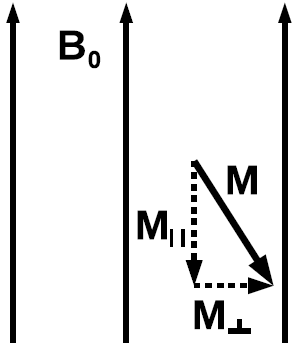
\includegraphics[height=35mm]{./Resources/magnetization_components.png}
		\caption{Zerlegung der Magnetisierung \autocite{skript}}
		\label{fig:mag_components}
	}
	%\hspace*{-20mm}  % fuegt Platz ein, das rueckt die beiden Bilder an den Rand
	\hspace*{\fill}
	\parbox{70mm}{
		\centering
		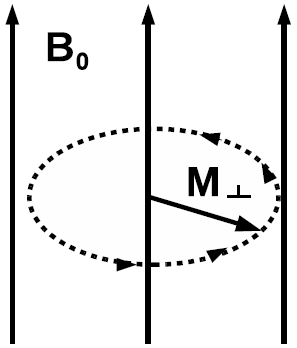
\includegraphics[height=35mm]{./Resources/larmor_precession.png}
		\caption{Larmor-Präzession von $M_{\perp}$ \autocite{skript}}
		\label{fig:larmor}
	}
\end{figure}

Im Grundzustand ist die Magnetisierung parallel zu den Feldlinien, in angeregten Zuständen können wir diese in einen Anteil $M_{\perp}$ senkrecht und $M_{\parallel}$ parallel zu den Feldlinien aufspalten (s. Abb. \ref{fig:mag_components}). Angeregte Zustände zerfallen dabei auf einer charakteristischen Zeitskala in den Grundzustand.

Die Wechselwirkung zwischen dem Magnetfeld $\vec{B_0}$ und der Magnetisierung $\vec{M}$ führt zu einem Drehmoment $\vec{\tau}$, wodurch $M_{\perp}$ mit einer Winkelfrequenz $\omega_{L}$ um $\vec{B_0}$ präzediert (s. Abb. \ref{fig:larmor}). Diese sogenannte Larmorfrequenz ist gegeben durch:
\begin{equation}
\omega_{L} = \gamma B_0
\label{eq:larmor_freq}
\end{equation}
\begin{figure}[H]
	\centering
	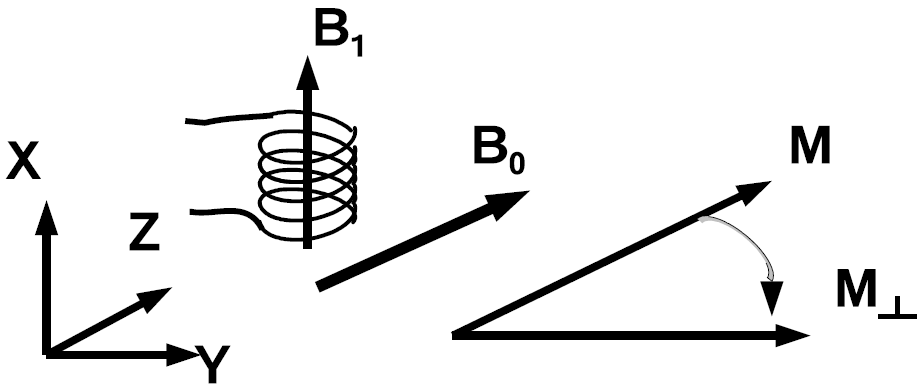
\includegraphics[width=70mm]{./Resources/hf_pulse.png}
	\caption{Hochfrequenzpuls zur Rotation der Magnetisierung \autocite{skript}}
\end{figure}
Eine bestimmte Magnetisierung kann durch Anlegen eines HF-Pulses an die Magnetisierung im Grundzustand erzeugt werden. Das zusätzliche Magnetfeld $\vec{B_1}$ dreht die Grundzustandsmagnetisierung während eines Zeitintervalls $\Delta t$ um einen Winkel
\begin{equation}
\alpha = \gamma B_1 \Delta t
\label{eq:pulseangle}
\end{equation}
Ist die Zeitdauer so gewählt, dass $\alpha = 90^\circ$ beträgt, wird $\vec{M}$ in eine senkrechte Komponente $M_{\perp}$ überführt ($90^\circ$-Puls). Ebenfalls kann durch $\alpha = 180^\circ$ eine Magnetisierung antiparallel zum statischen Feld $\vec{B_0}$ erzeugt werden ($180^\circ$-Puls).

\subsection{Kalibration des Systems}

An der Spule, auf die der HF-Puls gegeben wird, kann ebenfalls eine durch die präzedierende Magnetisierung hervorgerufene Induktionsspannung gemessen werden. Da dieses Signal mit der Larmorfrequenz $\omega_L$ moduliert ist, gibt eine Fouriertransformation Aufschluss über die Frequenzverteilung der Probe.
\newline\newline
Zunächst müssen die im Gerät als \texttt{PULS I} und \texttt{PULS II} ausgezeichneten Signalformen über die Pulsdauer als $90^\circ$- bzw $180^\circ$-Puls definiert werden. In Abbildung \ref{fig:pulse_signal} ist die Form eines solchen Pulses direkt nach dem Signalgenerator zu erkennen. Über die Potentiometer S6 und S7 ist die zeitliche Länge variierbar.

Um nun die Pulse zu kalibrieren, wird das in der Spule induzierte Signal auf dem Oszilloskop beobachtet (s. Abb. \ref{fig:pulse_induced}). \texttt{PULS I} entspricht genau dann einer Drehung um $90^\circ$, wenn die Anstiegsflanke des Pulses maximal steil ist, \texttt{PULS II} einer Drehung um $180^\circ$, wenn die Flanke möglichst flach ist.
\newline
\begin{figure}[H]
	\centering
	% hier schon der komplixiert Fall, dass 2 Bilder nebeneinander gesetzt werden
	\parbox{60mm}{
		\centering
		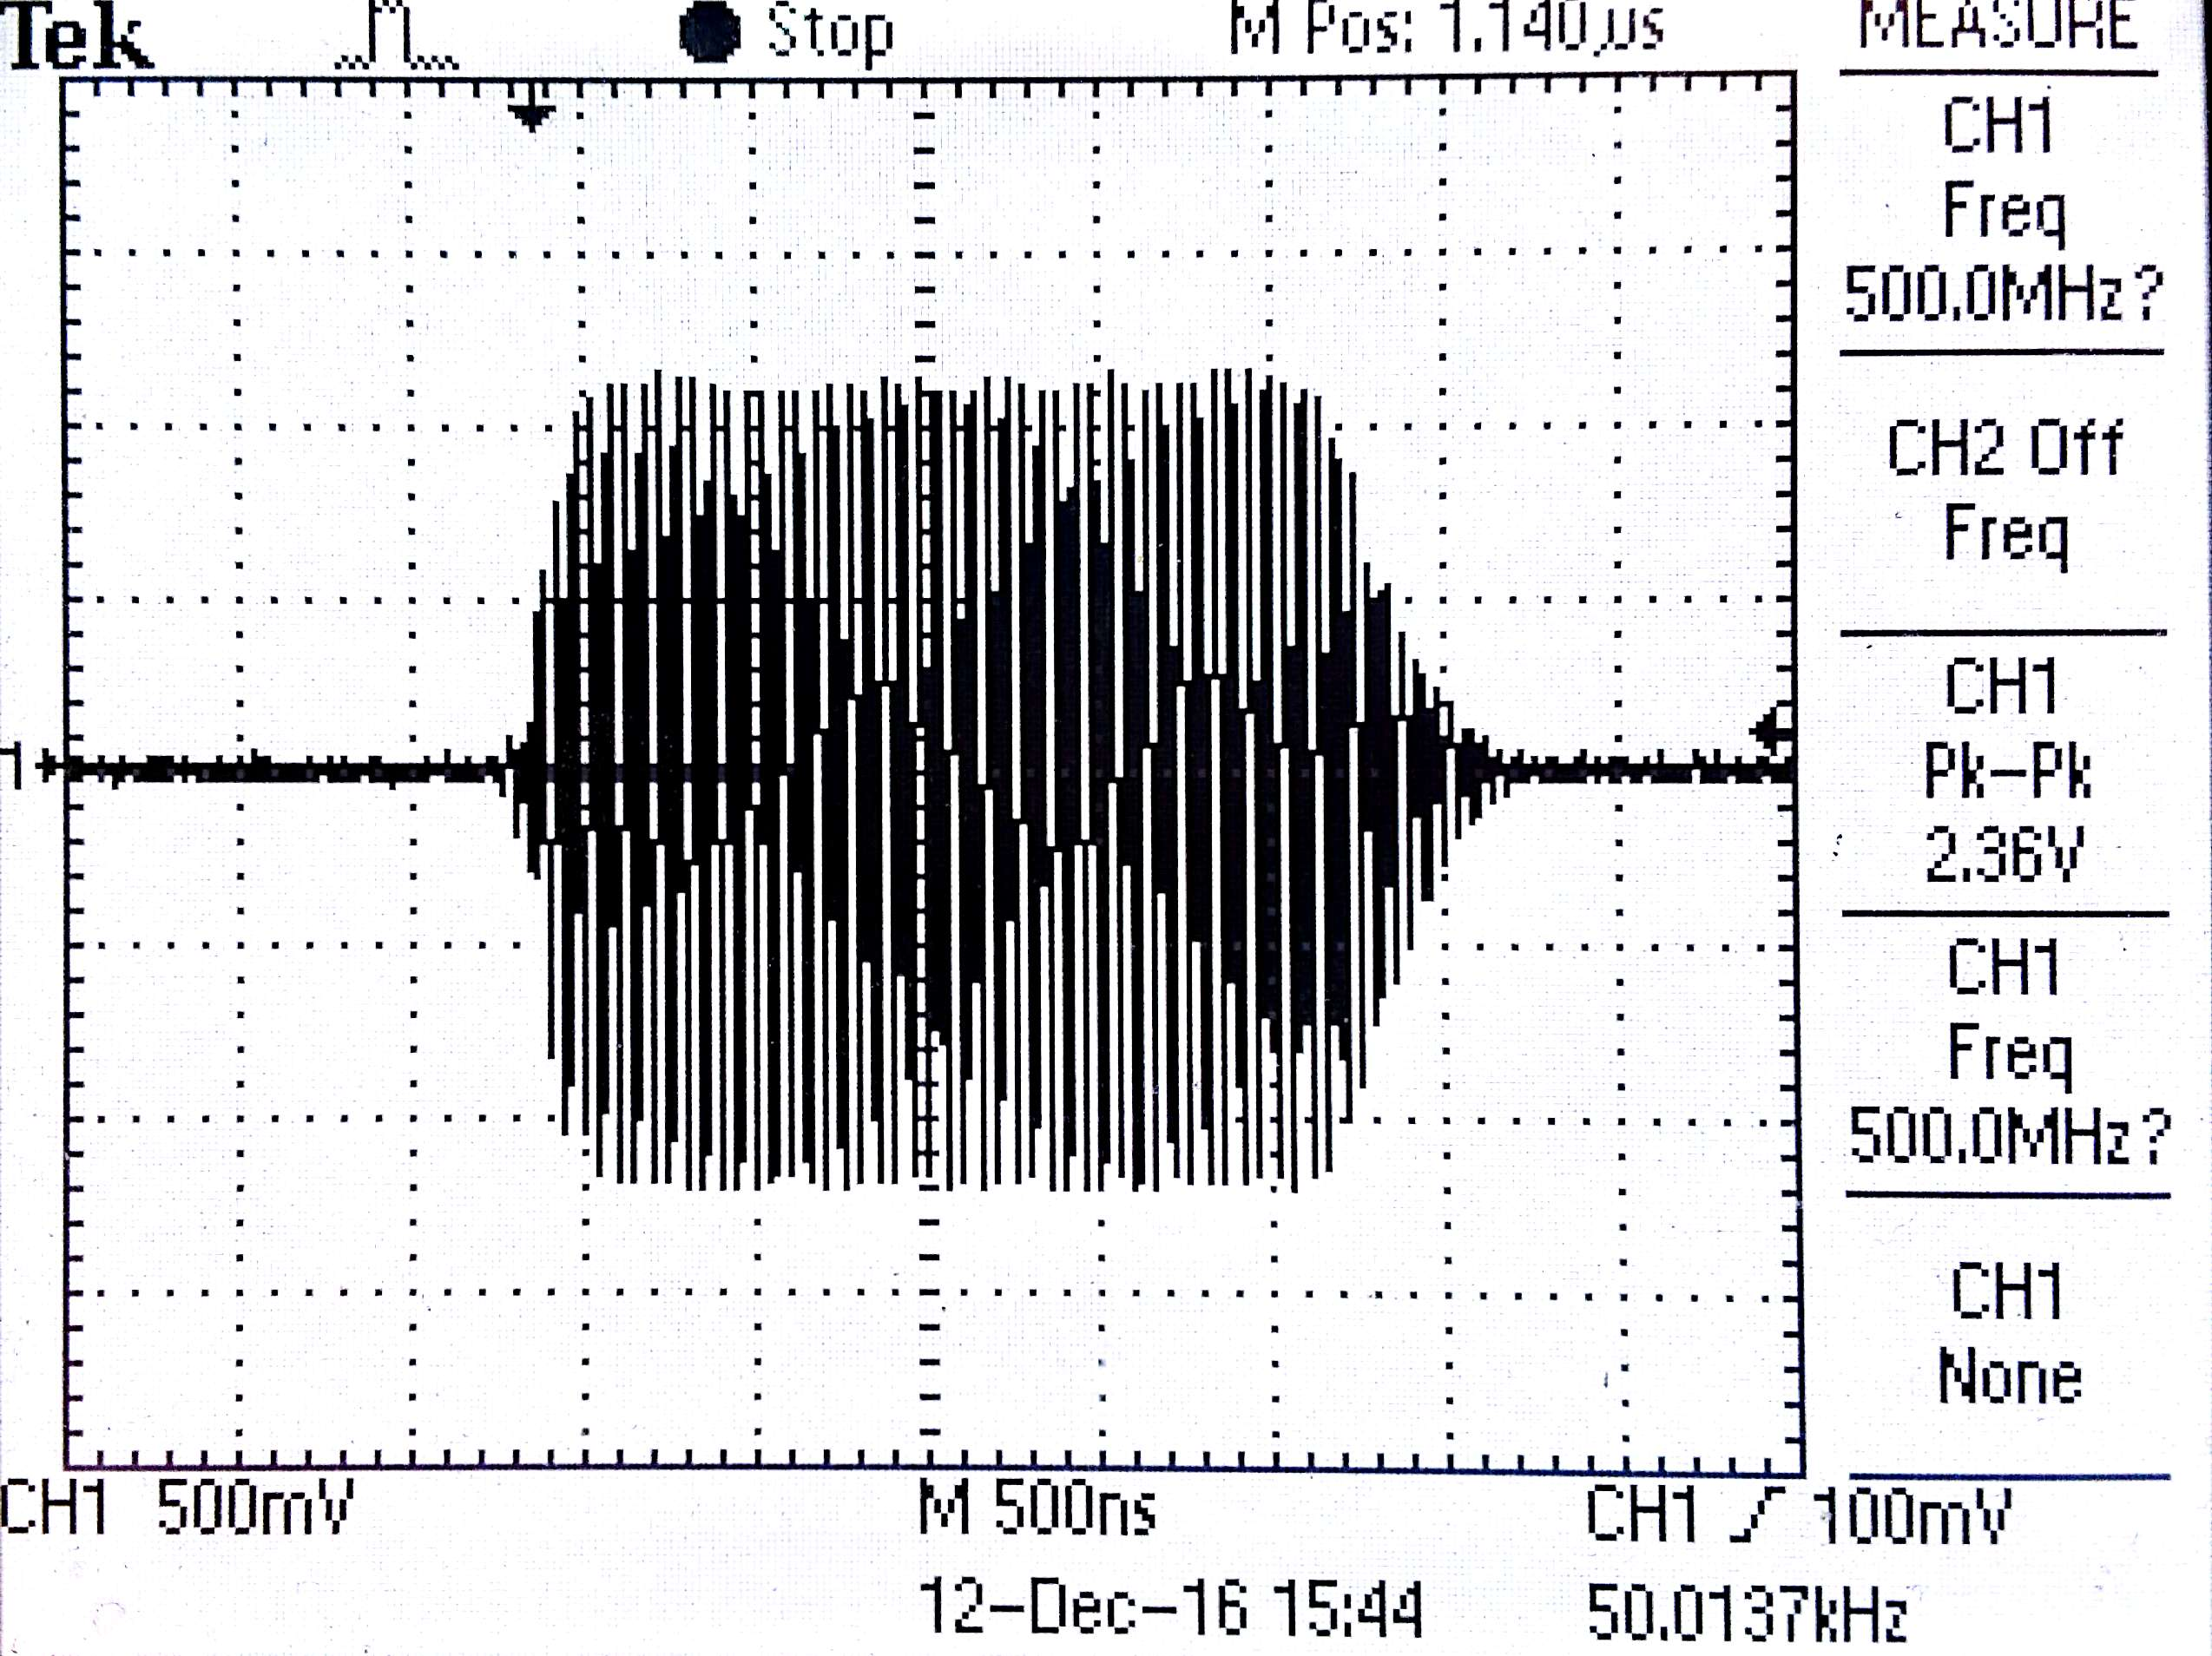
\includegraphics[width=55mm]{./Resources/pulse_train.jpg}
		\caption{Pulsform direkt nach dem Signalgenerator.}
		\label{fig:pulse_signal}
	}
	\hfill  % fuegt Platz ein, das rueckt die beiden Bilder an den Rand
	\parbox{60mm}{
		\centering
		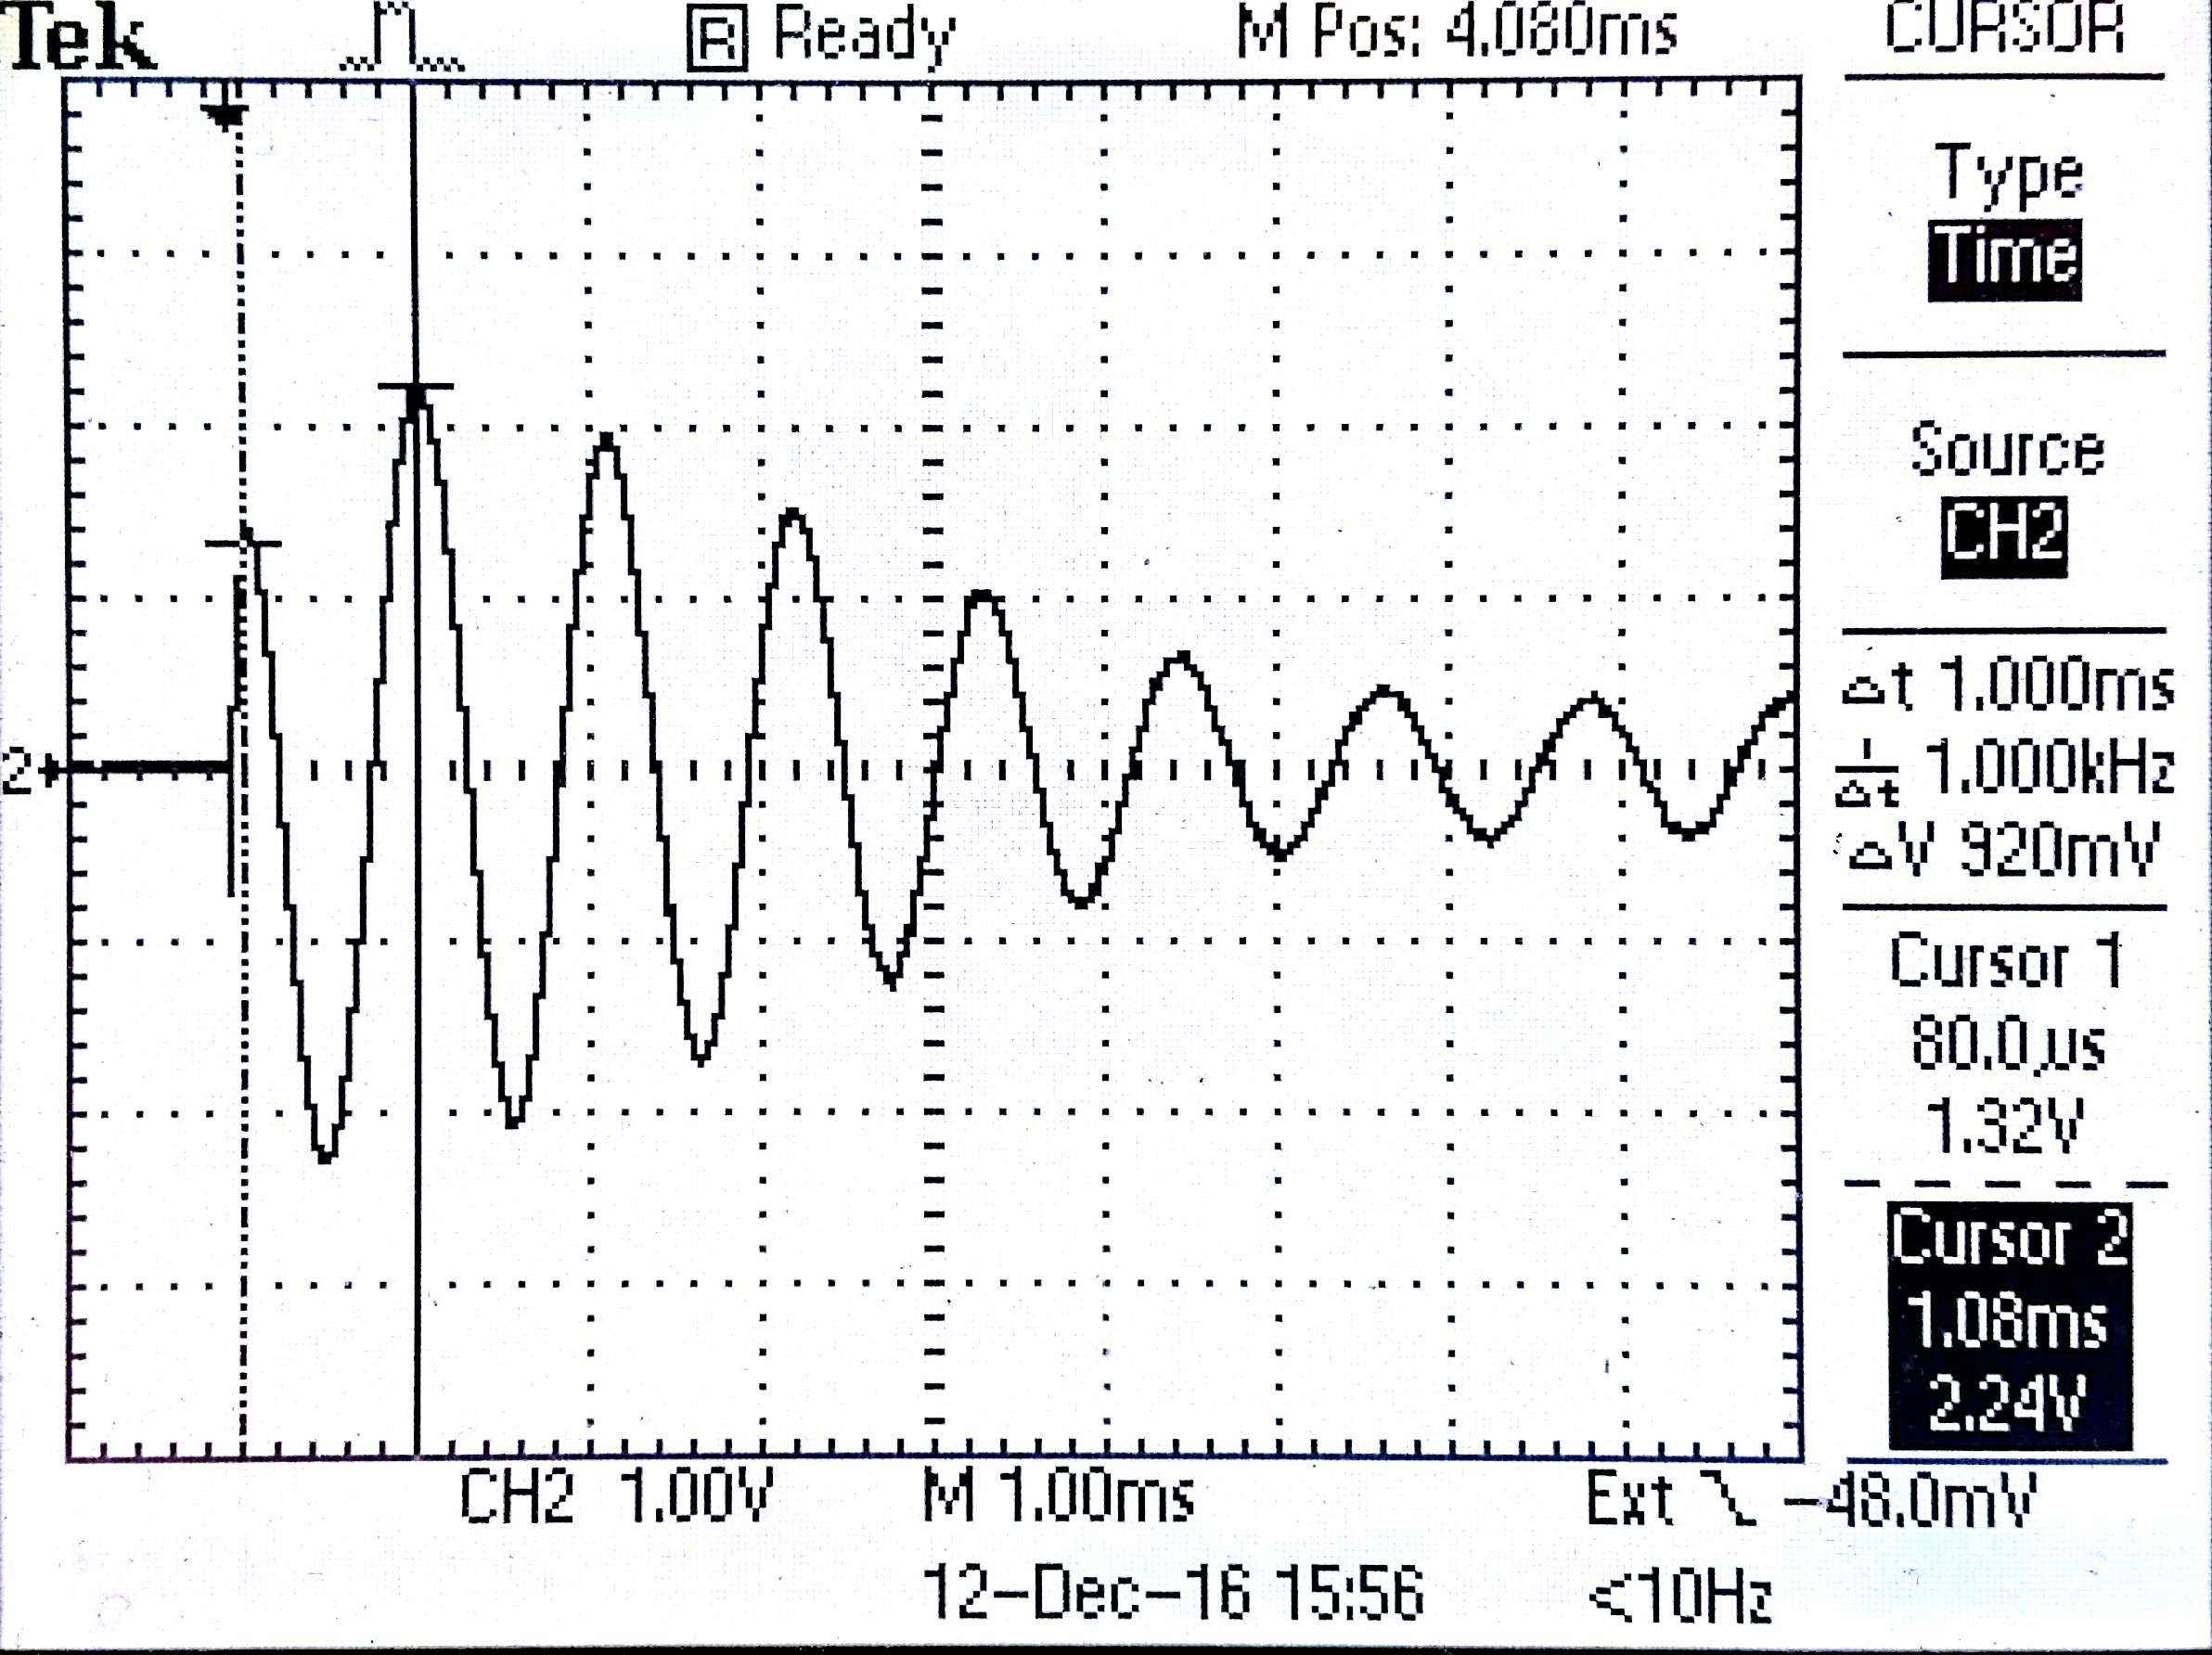
\includegraphics[width=55mm]{./Resources/single_pulse_event.jpg}
		\caption{Induziertes Signal in der Spule zur Pulskalibration.}
		\label{fig:pulse_induced}
	}
\end{figure}

Für die Kalibration wird Probe I (Gd 1:500 in Wasser) verwendet. Die HF-Pulse sind jeweils mit einer Frequenz von $\nu_{HF} = (19.9 \pm 0.2) \mhz$ moduliert. Die Arbeitsfrequenz wird nun durch Drehen der Schraube W1 auf $1\khz$ eingestellt. \texttt{PULS I} hat dann $90^\circ$-Verhalten, wenn $S6 \approx 2.0$ (Amplitude ca. $6V$), \texttt{PULS II} $180^\circ$-Verhalten, wenn $S7 \approx 2.1$ (Amplitude ca. $7V$). Über die FWHM des Pulses bestimmen wir die Pulsbreite zu:
\begin{itemize}
	\item[] \texttt{PULS I}: $t_1=\err{1,41}{0,10}\us$
	\item[] \texttt{PULS II}: $t_2=\err{2,48}{0,20}\us$
\end{itemize}

\section{Durchführung und Auswertung}

\subsection{Teil I: Relaxationszeiten}

\subsubsection{Theorie}

Relaxiert eine angeregte Magnetisierung zurück in den Grundzustand, so kann deren zeitliche Entwicklung durch die Bloch-Gleichungen beschrieben werden. In einem mitbewegten Bezugssystem sind diese gegeben durch:

\begin{equation}
\frac{dM_{\perp}(t)}{dt} = - \frac{M_{\perp}(t)}{T2}
\end{equation}
\begin{equation}
\frac{dM_{\parallel}(t)}{dt} = - \frac{M_{\parallel}(t) - M_0}{T1}
\end{equation}

Zur Energie eines angeregten Zustands tragen ma"sgeblich zwei verschiedene Wechselwirkungen bei. Der erste Anteil ist gegeben durch die Wechselwirkung der magnetischen Dipole mit dem externen Feld (Spin-Gitter Wechselwirkung). Zweitens interagieren auch die einzelnen Dipolmomente untereinander, wobei eine antiparallele Orientierung energetisch günstiger ist (Spin-Spin Wechselwirkung).

Die zeitliche Entwicklung einer transversalen Magnetisierung ergibt sich aus der Lösung von Gl. (4) zu:

\begin{equation}
M_{\perp}(t) = M_{\perp}^0 e^{-\frac{t}{T_2}}
\label{eq:spinrelax}
\end{equation}

Die Spin-Spin Relaxationszeit $T_2$ kann durch die sogenannte Spin-Echo Methode bestimmt werden (s. Abb. \ref{fig:spinecho_bloch}). Hierbei wird zunächst mit einem $90^\circ$-Puls eine transversale Magnetisierung erzeugt. Aufgrund des Magnetfelds $\vec{B_0}$ präzediert die Magnetisierung, wobei Protonen an unterschiedlichen aufgrund von Inhomogenitäten des Magnetfelds unterschiedliche Larmorfrequenzen haben. Zwei unterschiedliche Protonen haben dann zum Zeitpunkt $t=\tau$ eine Phasendifferenz aufgebaut, die durch Gabe eines $180^\circ$-Pulses umgekehrt werden kann. Nach der Zeit $t=2\tau$ sind die Magnetisierungen wieder in Phase, und das so erzeugte 'Spin-Echo' kann auf dem Oszilloskop beobachtet werden (s. Abb. \ref{fig:spinecho_osci}). Durch Messung des Maximums der Einhüllenden zu verschiedenen Zeiten $\tau$ können also einzelne Punkte des Zerfallsgesetztes (Gl. \ref{eq:spinrelax}) bestimmt werden.

 
Die Spin-Echo Methode wird für lange Zeiten zunehmend ungenau, da die Protonen vor Anlegen des $180^\circ$-Pulses an andere Positionen diffundieren können. Hierdurch kann nur teilweise Kohärenz erreicht werden; das Signal wird kleiner und wir messen zu niedrige Werte für $T_2$.

Diese Limitation kann durch Verwendung einer sogenannten Carr-Purcell Sequenz minimiert werden. Hierbei wird wie gehabt mit einem $90^\circ$-Puls angeregt, und nach allen ungeraden Vielfachen einer kurzen Zeit $\tau$ wird ein $180^\circ$-Puls auf die Spulen gegeben. Zu allen geraden Vielfachen von $\tau$ ist das System phasenkohärent, und wir können die Relaxation der Magnetisierung mit einer höheren Genauigkeit messen.

\begin{figure}[!htb]
	\centering
	% hier schon der komplixiert Fall, dass 2 Bilder nebeneinander gesetzt werden
	\parbox{70mm}{
		\centering
		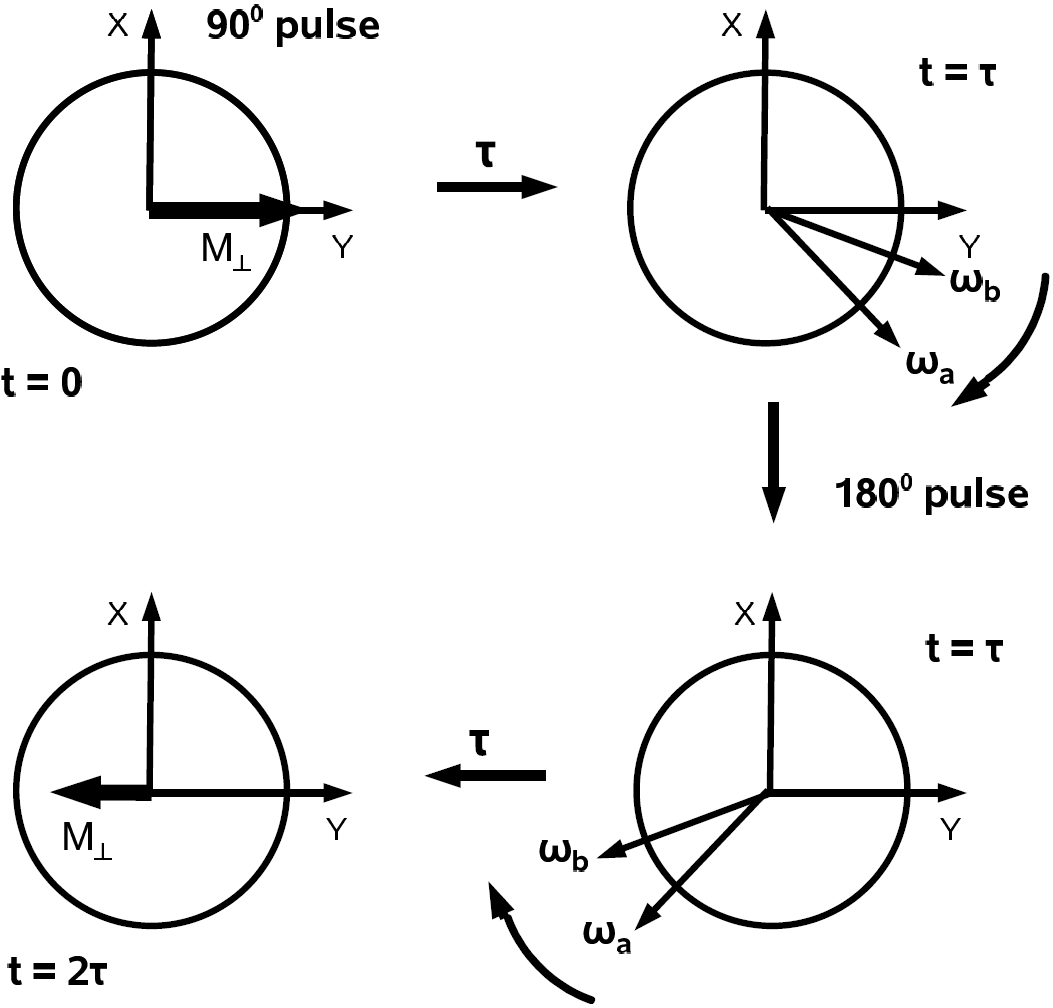
\includegraphics[height=50mm]{./Resources/spin_ech_schematic.png}
		\caption{Prinzip der Spin-Echo Methode \autocite{skript}}
		\label{fig:spinecho_bloch}
	}
	%\hspace*{-20mm}  % fuegt Platz ein, das rueckt die beiden Bilder an den Rand
	\hspace*{\fill}
	\parbox{70mm}{
		\centering
		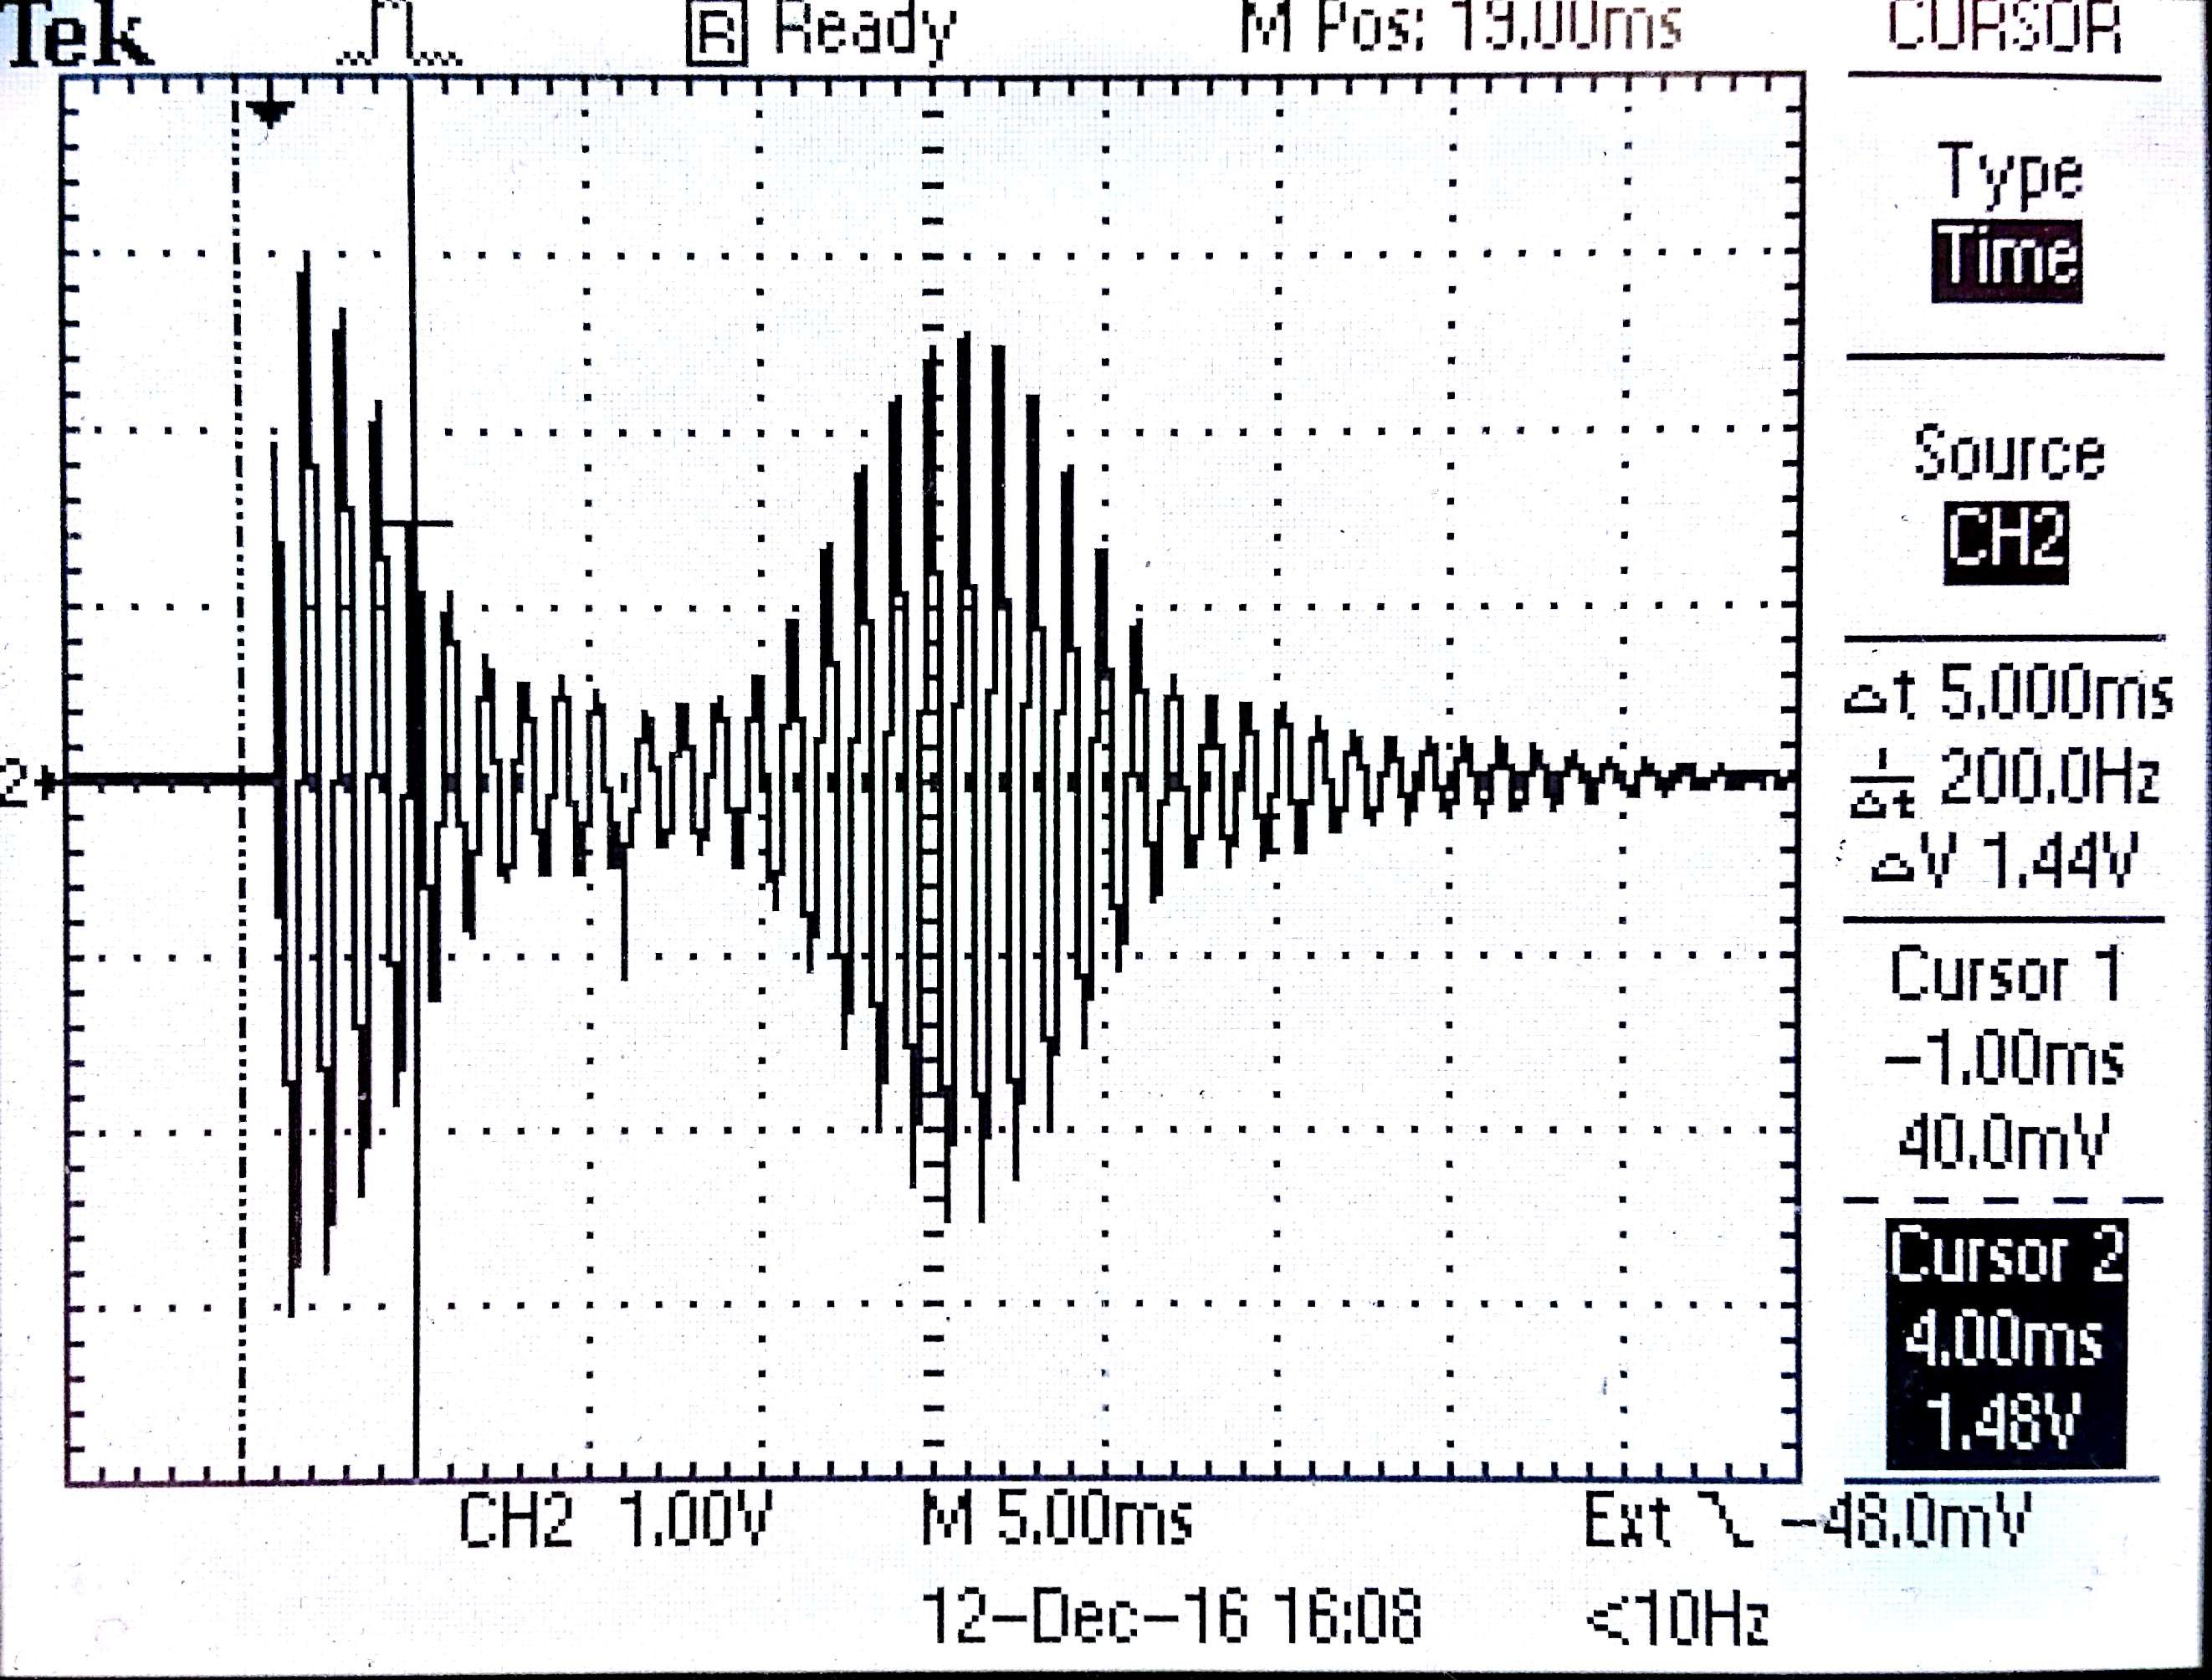
\includegraphics[height=50mm]{./Resources/spinecho_osci.jpg}
		\caption{Spin-Echo Messung mit $\tau=10ms$}
		\label{fig:spinecho_osci}
	}
\end{figure}

Die zeitliche Entwicklung einer antiparallelen Magnetisierung ergibt sich aus der Lösung von Gl. (5) zu:
\begin{equation}
M_{\parallel}(t) = M_{\parallel}^0(1-2e^{-\frac{t}{T_1}})
\end{equation}
Die Spin-Gitter Relaxationszeit $T_1$ kann bestimmt werden, in dem zunächst mit einem $180^\circ$-Puls angeregt wird. Diese Magnetisierung produziert kein Signal, weshalb nach einer Zeit $t=\tau$ ein $90^\circ$-Puls zur Messung auf die Spulen gegeben werden muss. Ähnlich der Spin-Echo Methode können nun einzelne Punkte der Zerfallskurve durch Messung bei variablen Werten von $\tau$ bestimmt werden.

\subsubsection{Durchführung}

Zunächst wird mithilfe der Spin-Echo Methode die Relaxationszeit $T_2$ bestimmt. Als Pulssequenz wählen wir die \texttt{I-II}-Folge mit $\tau = 10\ms$ und einer Wiederholrate von $1/3\hz$. Über ein LabView-Programm wird in einer Messreihe mit zehn Punkten die Amplitude der Spin-Echo-Einhüllenden als Funktion von $\tau$ gemessen. Das Programm ermittelt die Amplitude durch Transformation des Signals in den Frequenzraum, wobei für ein lineares Signal-zu-Rausch Verhältnis (SNR) jeweils automatisch über zehn Messungen gemittelt wird. Weil die Trial-to-trial variability zum Teil deutlich größer als die angegebene Standardabweichung war, haben wir jeden Datenpunkt mehrmals gemessen.

Für Probe 1 (Gd 1:500) ergibt sich durch exponentiellen Fit (s. Abb. \ref{fig:t2_p1}):
\begin{enumerate}
	\item[] $T_2 = \err{119,5}{0,5} \ms$
	\item[] $A = \err{8,6}{0,0} \be$
\end{enumerate}
Analog dazu ergibt sich für Probe 3 (Gd 1:600) (s. Abb. \ref{fig:t2_p3}):
\begin{enumerate}
	\item[] $T_2 = \err{139,3}{0,8} \ms$
	\item[] $A = \err{8,1}{0,0} \be$
\end{enumerate}
\begin{figure}[H]
	\centering
	% hier schon der komplixiert Fall, dass 2 Bilder nebeneinander gesetzt werden
	\parbox{70mm}{
		\centering
		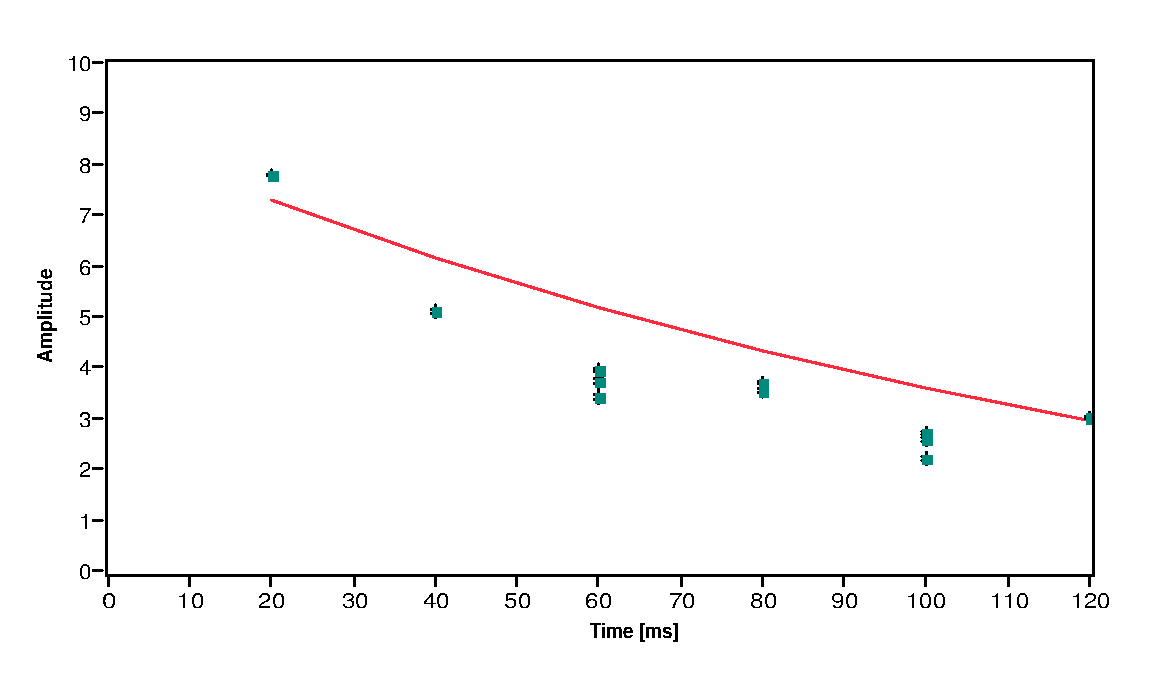
\includegraphics[width=70mm]{./Resources/t2_meas_p1.eps}
		\caption{T2-Messung Probe 1 mit Fit.}
		\label{fig:t2_p1}
	}
	%\hspace*{-20mm}  % fuegt Platz ein, das rueckt die beiden Bilder an den Rand
	\hspace*{\fill}
	\parbox{70mm}{
		\centering
		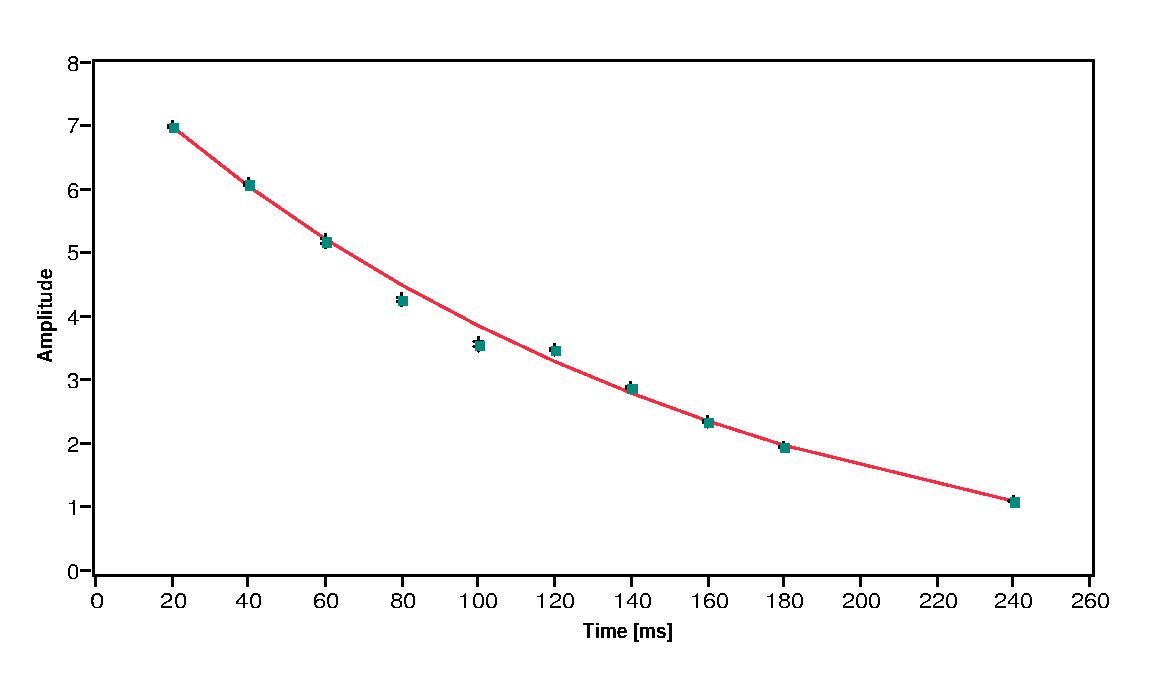
\includegraphics[width=70mm]{./Resources/t2_meas_p3.eps}
		\caption{T2-Messung Probe 3 mit Fit.}
		\label{fig:t2_p3}
	}
\end{figure}

Zum Vergleich wird die Relaxationszeit $T_2$ mittels einer Carr-Purcell-Sequenz gemessen. Im LabView-Programm wird über 10 Messungen gemittelt, die Zeitdifferenz zwischen den Pulsen beträgt $\tau = 20\ms$.

Für Probe 1 (Gd 1:500) ergibt sich durch exponentiellen Fit (s. Abb. \ref{fig:t2_p1_cp}):
\begin{enumerate}
	\item[] $T_2 = \err{140,1}{0,4} \ms$
	\item[] $A = \err{92,8}{0,4} \be$
\end{enumerate}
Analog dazu ergibt sich für Probe 3 (Gd 1:600) (s. Abb. \ref{fig:t2_p3_cp}):
\begin{enumerate}
	\item[] $T_2 = \err{166,9}{0,4} \ms$
	\item[] $A = \err{93,9}{0,2} \be$
\end{enumerate}

\begin{figure}[H]
	\centering
	% hier schon der komplixiert Fall, dass 2 Bilder nebeneinander gesetzt werden
	\parbox{70mm}{
		\centering
		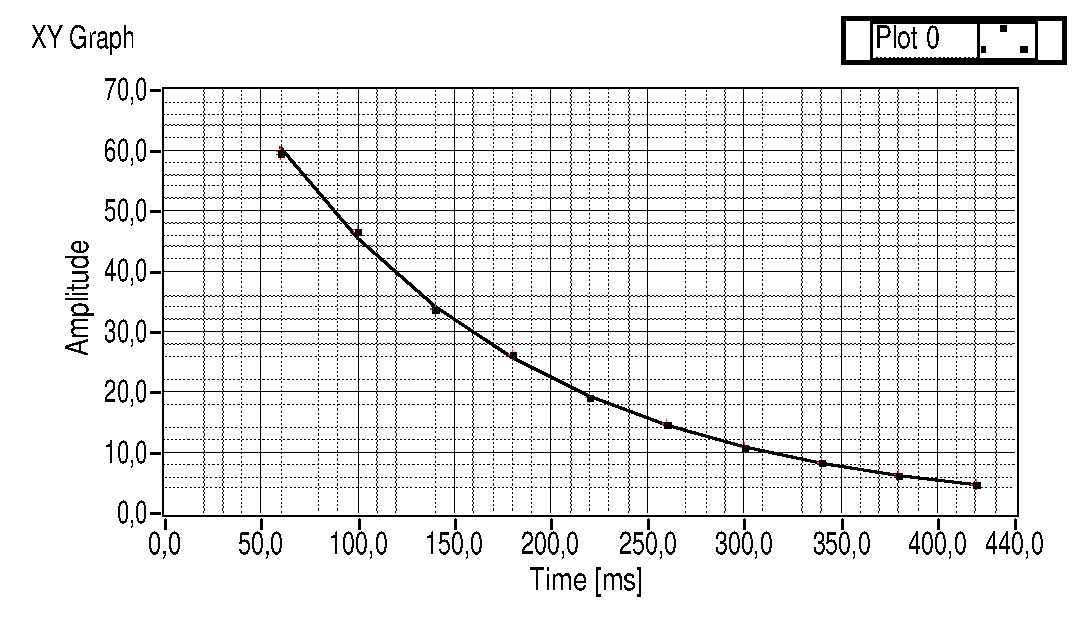
\includegraphics[width=70mm]{./Resources/t2_p1_cp.eps}
		\caption{T2-Messung über Carr-Purcell Probe 1 mit Fit.}
		\label{fig:t2_p1_cp}
	}
	%\hspace*{-20mm}  % fuegt Platz ein, das rueckt die beiden Bilder an den Rand
	\hspace*{\fill}
	\parbox{70mm}{
		\centering
		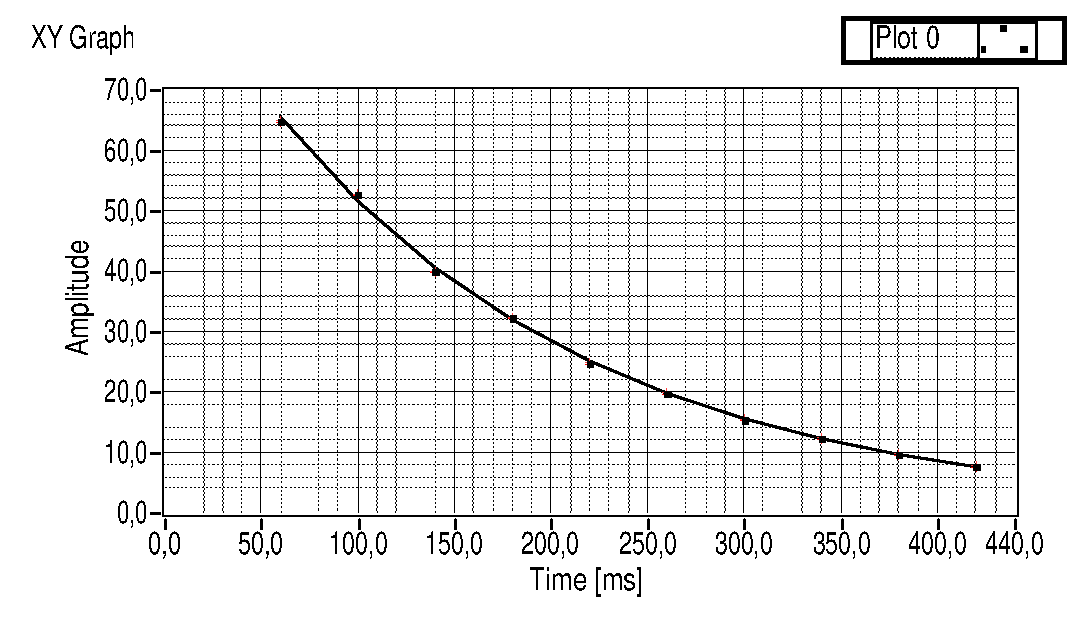
\includegraphics[width=70mm]{./Resources/t2_p3_cp.eps}
		\caption{T2-Messung über Carr-Purcell Probe 3 mit Fit.}
		\label{fig:t2_p3_cp}
	}
\end{figure}
Anschließend wird die Spin-Gitter Relaxationszeit $T_1$ bestimmt, wobei das Messprinzip identisch zur ersten Messung von $T_2$ ist. Die Parameter bleiben unverändert.

Für Probe 1 (Gd 1:500) ergibt sich durch exponentiellen Fit (s. Abb. \ref{fig:t1_p1}):
\begin{enumerate}
	\item[] $T_1 = \err{125,5}{0,6} \ms$
	\item[] $A = \err{3,79}{0,02} \be$
\end{enumerate}
Analog dazu ergibt sich für Probe 3 (Gd 1:600) (s. Abb. \ref{fig:t1_p3}):
\begin{enumerate}
	\item[] $T_1 = \err{150,5}{1,2} \ms$
	\item[] $A = \err{4,17}{0,03} \be$
\end{enumerate}

\begin{figure}[H]
	\centering
	% hier schon der komplixiert Fall, dass 2 Bilder nebeneinander gesetzt werden
	\parbox{70mm}{
		\centering
		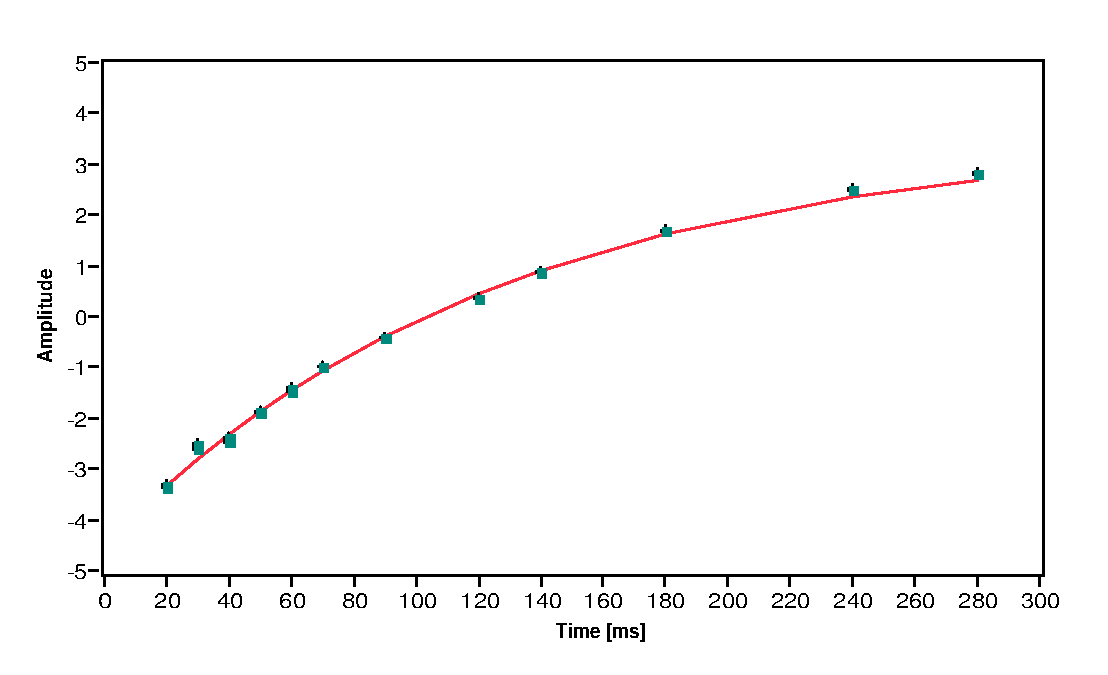
\includegraphics[width=70mm]{./Resources/t1_meas_p1.eps}
		\caption{T1-Messung Probe 1 mit Fit.}
		\label{fig:t1_p1}
	}
	%\hspace*{-20mm}  % fuegt Platz ein, das rueckt die beiden Bilder an den Rand
	\hspace*{\fill}
	\parbox{70mm}{
		\centering
		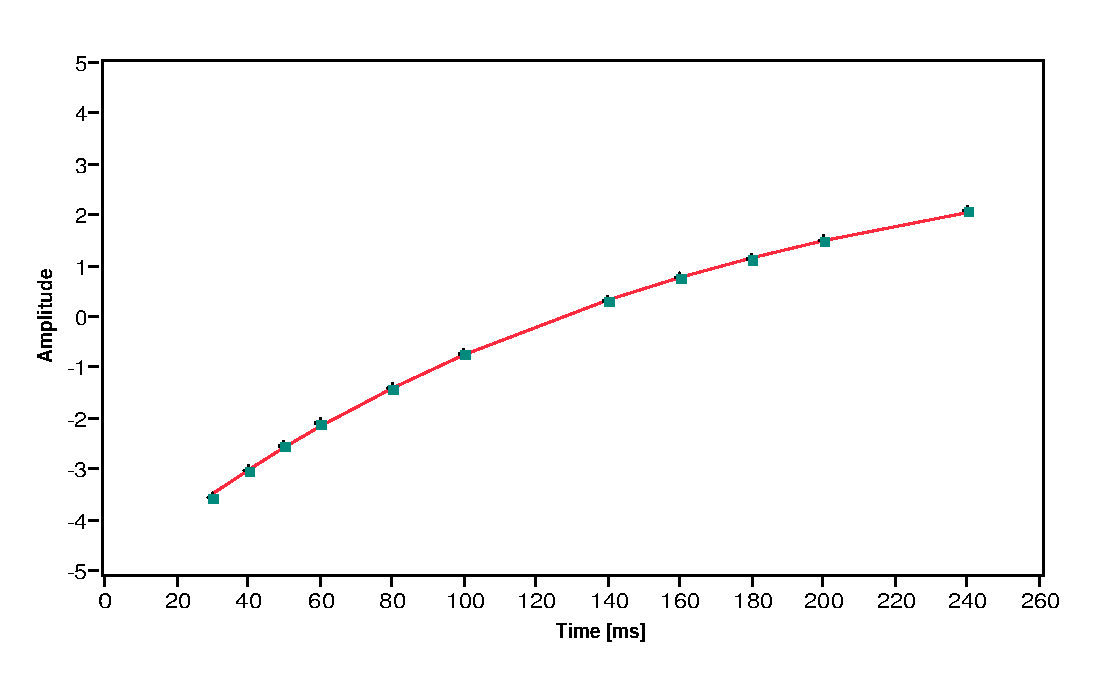
\includegraphics[width=70mm]{./Resources/t1_meas_p3.eps}
		\caption{T1-Messung Probe 3 mit Fit.}
		\label{fig:t1_p3}
	}
\end{figure}

\subsubsection{Auswertung}

In Tabelle \ref{tab:relaxtimes} sind unsere Messungen für die Relaxationszeiten $T_1$ und $T_2$ zusammengefasst.

\begin{table}[H] 
	\centering
	\caption{Strukturparameter der Kalibrationsgitter}
	\label{tab:relaxtimes}
	\begin{tabular}{cccc}
		\toprule
		Zeit & $T_1$ [$\mathrm{ms}$] & $T_2$ [$\mathrm{ms}$] & $T_2$ [$\mathrm{ms}$]\\
		Methode & Spin-Echo & Spin-Echo & Carr-Purcell\\
		\midrule
		Probe 1 (Gd 1:500)& $\err{125,5}{0,6}$ & $\err{119,5}{0,5}$ & $\err{140,1}{0,4}$\\
		Probe 3 (Gd 1:600)& $\err{150,5}{1,2}$ & $\err{139,3}{0,8}$ & $\err{166,9}{0,4}$\\
		\bottomrule
	\end{tabular}
\end{table}

Zunächst fällt bei den Messungen für $T_2$ auf, dass die Messwerte über die Carr-Purcell Sequenz für beide Proben größer als über die Spin-Echo Methode sind. Da die Carr-Purcell Methode Inhomogenitäten des Magnetfeldes korrigiert, erwarten wir, dass diese Messungen näher an den wahren Werten liegen.
Laut Theorie der Relaxationsvorgänge ist die Interaktion zwischen verschiedenen Spins aufgrund des größeren Winkels zueinander höher als die Interaktion zwischen Spin und Gitter. Somit sollte die Zerfallszeit $T_2$ kleiner als $T_1$ sein (stärkere Kopplung bedingt schnelleren Zerfall), was aber nur für die Messungen mit der Spin-Echo Methode gegeben ist. Die Zeitkonstanten für die stärker verdünnte Probe 3 sind allesamt größer, was auch direkt durch die höhere Konzentration von Wasserstoffkernen ersichtlich ist.

Um die Genauigkeit der Messungen zu steigern, sollten einige systematische Fehlerquellen eliminiert werden: Zunächst ist die Arbeitsfrequenz durch Temperaturerhöhung während des Versuchs stark gedriftet. Daher mussten wir über die Einstellschraube am Gehäuse mehrfach nachkorrigieren, wodurch sicherlich Ungenauigkeiten entstanden sind. Abhilfe würde eine bessere thermische Isolierung und ein automatisierter Messprozess bieten, der die absolute Messdauer reduziert und somit Temperaturdrifts verringert. Ebenfalls war es nur unzureichend möglich, die Pulsdauern genau einzustellen. Vor allem bei dem $180^\circ$-Puls war die Differenz zwischen maximaler und minimaler Amplitude sehr klein, und das Signal ist auch nicht komplett auf Null abgefallen. Hierdurch ist die Projektion der Magnetisierung sowie das Umkehren der Phasenwinkel mit einem großen Fehler behaftet, was sicherlich zu einer signifikanten Ungenauigkeit führt. Als Probemlösung ist die Verwendung einer digitalen Einstellmöglichkeit, anstatt der nur grob einstellbaren, analogen Drehregler, vorzuschlagen. Eventuell könnte diese Einstellung sogar automatisiert über eine Regelschleife erfolgen, um die optimalen Pulsdauern zu finden.

Zum Abschluss schätzen wir aus den gemessenen Arbeitsfrequenzen und Pulsdauern die Feldstärken der beiden Magnetfelder. Aus der Larmorfrequenz (Gl. \ref{eq:larmor_freq}) lässt sich unter der Näherung $\omega_{L} \approx \omega_{HF} = 2\pi \nu_{HF} = 2\pi \times \err{19.9}{0.2}\mhz$ die Feldstärke des statischen Feldes bestimmen:
\begin{itemize}
\item[] $B_0 = \err{0.467}{0.002}\mathrm{T}$
\end{itemize}
Aus den Drehwinkeln der beiden Pulse zusammen mit ihrer gemessenen Dauer (s. Kap. 1.2) ergibt sich dann über Gl. \ref{eq:pulseangle} die Feldstärke des Wechselfeldes zu:
\begin{itemize}
	\item[] $B_1 \approx 0.3\mathrm{mT}$ (aus beiden Pulsen)
\end{itemize}
Beide Feldstärken erscheinen physikalisch sinnvoll; Referenzwerte für diese Apparatur lagen leider nicht vor.

\subsection{Teil II: Chemische Verschiebung}

\subsubsection{Theorie}

Im folgenden Abschnitt betrachten wir Protonen, die in Molekülen gebunden sind. In diesem Fall wird das äußere Magnetfeld $B_0$ aufgrund der Elektronenorbitale in der Umgebung des Protons um den Betrag

\begin{equation}
	\delta \vec{B} = - \sigma \vec{B_0}
	\label{eq:delta_B}
\end{equation}

verringert. Nach Gleichung \eqref{eq:larmor_freq} wird dadurch auch die Larmorfrequenz modifiziert:

\begin{equation}
	\omega_i = \omega_L \left(1-\sigma_i \right)
	\label{eq:omega_i}
\end{equation}

Der Proportionalitätsfaktor $\sigma$ repräsentiert dabei die magnetische Abschirmung und ist charakteristisch für die chemische Gruppe, in der sich das Proton befindet. Damit ist die Messung von $\omega_i$ für die chemische Strukturanayse von Substanzen geeignet.

\begin{wrapfigure}[10]{r}{0.2\textwidth}
	\begin{center}
		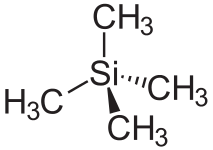
\includegraphics[width = 0.18\textwidth]{./Resources/Tetramethylsilan.png}
	\end{center}
  \caption{Te\-tramethylsilan}
  \label{fig:TMS}
\end{wrapfigure}

Um chemische Substanzen zu identifizieren, wird der Probe eine Referenzsubstanz beigemischt. Alle \emph{chemischen Verschiebungen}, also Verschiebungen der Larmorfrequenz $\omega_{L}$ aufgrund der Elekronenorbitale, werden relativ zu dieser Referenz angegeben. Für diesen Zweck hat sich \emph{Tetramethylsilan (TMS)} \autocite{TMS} (siehe Abbildung \ref{fig:TMS}) etabliert, da es weitgehend chemisch inert ist, und einen einzigen starken Peak im Spektrum liefert. Außerdem hat es wegen der geringen chemischen Elektronegativität von Silizium eine kleinere Frequenz als die meisten funktionellen Gruppen der organischen Chemie, weshalb der Wert für $\delta_i$ in der Regel positiv (siehe Abbildung \ref{fig:chem_shift}) ist. Es ist üblich, die relative Verschiebung der Frequenz in der Einheit ppm (parts per million) anzugeben.

\begin{equation}
	\delta_i = \sigma_i -\sigma_{TMS} = \frac{\omega_{TMS} - \omega_i}{\omega_L}
	\label{eq:delta_i}
\end{equation}

Dies hat den Vorteil, dass die Werte für die chemischen Verschiebungen unabhängig vom angelegten Magnetfeld $B_0$ sind, und damit die Messergebnisse unterschiedlicher Messapparaturen miteinander vergleichbar sind.
In Abbildung \ref{fig:chem_shift} sind die chemischen Verschiebungen für diverse organische Verbindungen dargestellt.

\begin{figure}[htbp]
	\centering
	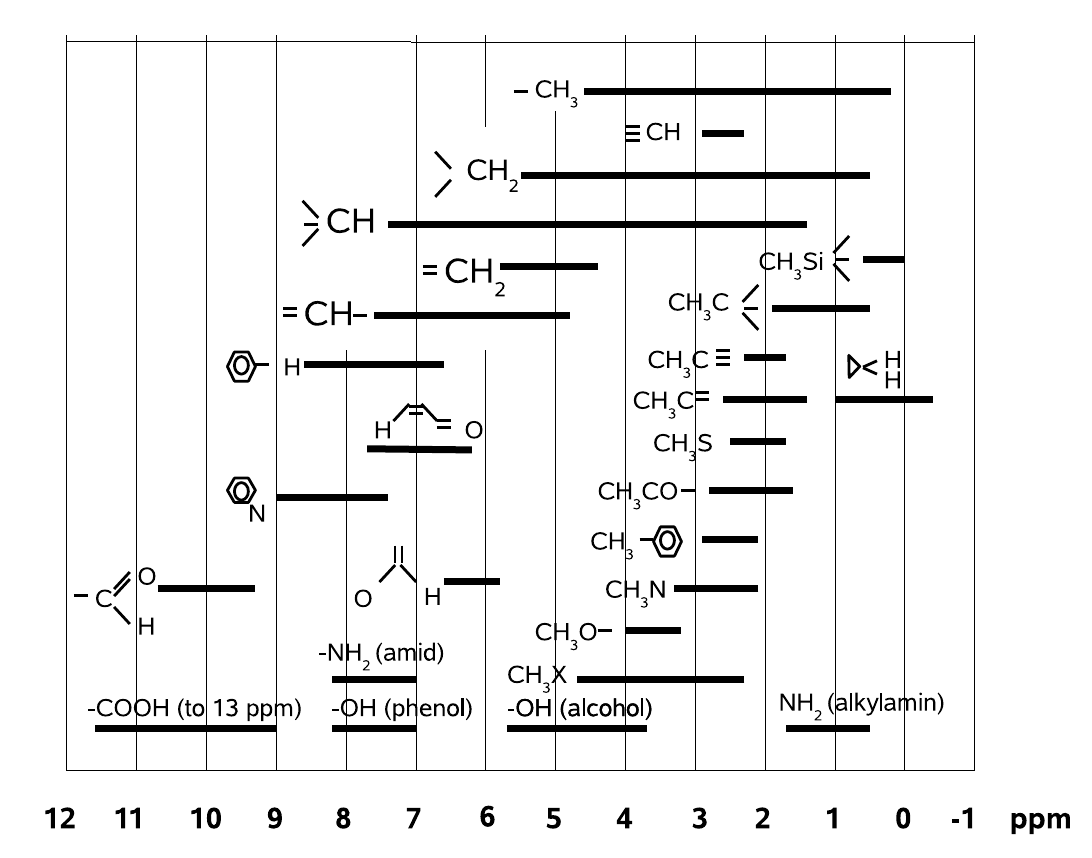
\includegraphics[width= 0.9\textwidth]{./Resources/chem_shifts.png}
	\caption{Chemische Verschiebung $\delta_i$ verschiedener funktioneller Gruppen relativ zu TMS \autocite{skript}}
	\label{fig:chem_shift}
\end{figure}


\subsubsection{Durchführung}

Das Ziel dieses Versuchsteils war die Identifizierung von verschiedenen chemischen Substanzen anhand ihrer chemischen Verschiebung. Als Referenz haben wir das oben erwähnte TMS verwendet. Allgemein standen uns jeweils fünf chemische Proben in zweifacher Ausführung zur Verfügung: einmal die reine Substanz und einmal ein Gemsich aus der Substanz und TMS. Zusätzlich muss die Probe, die in einem dünnen Glasrohr eingeschlossen ist, mittels Druckluft in Rotation versetzt werden, um die Schärfe der Messpeaks bzw. die Auflösung zu optimieren. Inhomogenitäten in der Probe und im Magnetfeld $B_0$ sowie Diffusionsprozesse verschlechtern die Auflösung. Das Spektroskop wird bei einer Working-Frequency von $\nu_{\omega} = $ \SI{500}{Hz} und mit $90^{\circ}$ - Pulsen bei einer Wiederholrate von \SI{1/3}{Hz}.

\paragraph{Einfluss der Rotation}

Zunächst untersuchen wir, welchen Einfluss die Rotation der Proben auf das Messergebnis hat. Dazu wird Probe 3 verwendet. Ohne Rotation hat das Responsesignal eine Breite (FWHM) von ca. \SI{200}{Hz} bei einer maximalen Intensität von 0,25. Mit Rotation beträgt die Breite nur ca. \SI{20}{Hz} und das Maximum 1,9. Offensichtlich lässt sich also die Breite der Peaks und damit die Auflösung durch diese Methode deutlich verbessern, weil sich die oben genannten Inhomogenitäten und Diffusionseffekte herausmitteln.

\paragraph{Zuordnung der Proben}
Wir messen nacheinander die Präparate A bis E, jeweils mit TMS-Beimischung\footnote{Die Daten für die Proben A+ und D+ stammen aus der Datenbank, da uns keine Probe zur Verfügung stand} (gekennzeichnet durch ein +) und ohne. Der relative Abstand der Peaks, die zu den chemischen Gruppen gehören, gibt Aufschluss über die chemische Zusammensetzung. Uns standen folgende Proben zur Verfügung:

\begin{description}
	\item[Toluol] 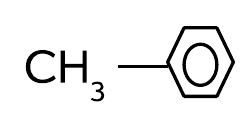
\includegraphics[height = 0.6 cm]{./Resources/toluol.png}
	\item[p-Xylol] 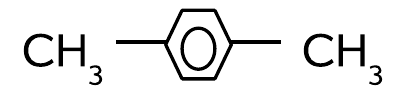
\includegraphics[height = 0.6 cm]{./Resources/p-xylol.png}
	\item[Essigsäure] 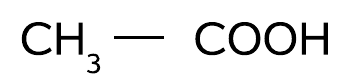
\includegraphics[height = 0.6 cm]{./Resources/acetic_acid.png}
	\item[Fluoraceton] 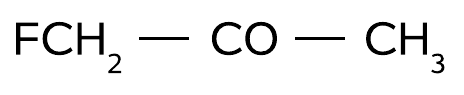
\includegraphics[height = 0.6 cm]{./Resources/fluoroacetone.png}
	\item[Fluoroacetonitril] 
\includegraphics[height = 0.6 cm]{./Resources/fluoroacetonitril.png}
\end{description}

Unsere Messergebnisse sind in den Talleben \ref{tab:Probe_A} bis \ref{tab:Probe_E} zusammen mit der Zuordnung zu der entsprechenden chemischen Gruppe dargestellt.



\begin{table}[!htb]
	\centering
	\caption{Messergebnisse für Probe A, Zuordnung: \emph{Flouraceton} }
	\label{tab:Probe_A}
	\begin{tabularx}{1.0\linewidth}{cccX}
	\toprule
	Peaks von A+ [ppm] & Peaks von A [ppm] & Chem. Versch. & Zuordnung \\
	\midrule
	$p_1 = 22,2$ & $p_1 = 23,8$ & $\delta_i = 6,3$ & \multirow{2}{*}{\ce{FCH2}-Gruppe} \\

	$p_2 = 24,6$ & $p_2 = 21,4$ & $\delta_i= 3,9$ &  \\

	$p_3 = 26,4$ & $p_3 = 19,6$ & $\delta_i = 2,1 $ & Methyl-Gruppe \ce{CH3} \\

	$p_4 = 28,5$ & -- & -- & TMS \\
	\bottomrule
	\end{tabularx}


\end{table}

\begin{table}[!htb]
	\centering
	\caption{Messergebnisse für Probe B, Zuordnung: \emph{p-Xylol} }
	\label{tab:Probe_B}
	\begin{tabularx}{1.0\linewidth}{cccX}
	\toprule
	Peaks von B+ [ppm] & Peaks von B [ppm] & Chem. Versch. & Zuordnung \\
	\midrule
	$p_1 = 22,7$ & $p_1 = 22,7$ & $\delta_i = 7,0$ & Benzol-Gruppe \\

	$p_2 = 27,5$ & $p_2 = 27,5$ & $\delta_i = 2,2$ & Methyl-Gruppe, Peak doppelt so groß wie $p_1$ \\

	$p_3 = 29,7$ & -- & --  & TMS \\

	\bottomrule
	\end{tabularx}


\end{table}

\begin{table}[!htb]
	\centering
	\caption{Messergebnisse für Probe C, Zuordnung: \emph{Essigsäure} }
	\label{tab:Probe_C}
	\begin{tabularx}{1.0\linewidth}{cccX}
	\toprule
	Peaks von C+ [ppm] & Peaks von C [ppm] & Chem. Versch. & Zuordnung \\
	\midrule
	$p_1 = 16,7$ & $p_1 = 17,0$ & $\delta_i = 11,6$ & \ce{COOH}-Gruppe \\

	$p_2 = 26,2$ & $p_2 = 26,6$ & $\delta_i = 2,1$ & Methyl-Gruppe \ce{CH3} \\

	$p_3 = 28,3$ & -- & -- & TMS \\
	\bottomrule
	\end{tabularx}


\end{table}

\begin{table}[!htb]
	\centering
	\caption{Messergebnisse für Probe D, Zuordnung: \emph{Fluoroacetonitril} }
	\label{tab:Probe_D}
	\begin{tabularx}{1.0\linewidth}{cccX}
	\toprule
	Peaks von D+ [ppm] & Peaks von D [ppm] & Chem. Versch. & Zuordnung \\
	\midrule
	$p_1 = 30,8$ & -- & -- & TMS \\

	$p_2 = 34,8$ & $p_2 = 26,6$ & $\delta_i = 6,4$ & \multirow{2}{*}{\ce{FCH2}-Gruppe} \\

	$p_3 = 37,2$ & $p_3 = 24,2$ & $delta_i = 4,0$ &  \\

	\bottomrule
	\end{tabularx}

\end{table}

\begin{table}[!htb]
	\centering
	\caption{Messergebnisse für Probe E, Zuordnung: \emph{Toluol} }
	\label{tab:Probe_E}
	\begin{tabularx}{1.0\linewidth}{cccX}
	\toprule
	Peaks von E+ [ppm] & Peaks von E [ppm] & Chem. Versch. & Zuordnung \\
	\midrule
	$p_1 = 19,5$ & $p_1 = 23,1$ & $\delta_i = 7,3 $ & Benzol-Gruppe \\

	$p_2 = 24,4$ & $p_2 = 23,1$ & $\delta_i = 2,4$ & Methyl-Gruppe, beide Peaks gleich groß \\

	$p_3 = 26,8$ & -- & -- & TMS \\

	\bottomrule
	\end{tabularx}

\end{table}

\subsubsection{Auswertung}
\paragraph{Zuordnung}

Bei der Zuordnung sind wir nach dem Ausschlussprinzip vorgegangen. Probe C lässt sich eindeutig der \emph{Essigsäure} zuweisen, da die COOH-Gruppe gemäß Abbildung \ref{fig:chem_shift} eine sehr charakteristische hohe chemische Verschiebung von \SI{9}{ppm} bis \SI{13}{ppm} hat. Wegen der hohen Elektronegativität des Sauerstoffatoms wird das Elektron des Wasserstoffs stark vom Protonkern weggezogen, was den hohen Wert dür $\delta_i$ erklärt.
Die Stoffe \emph{Toluol} und \emph{p-Xylol} sind in ihrem chemischen Aufbau sehr ähnlich, mit dem Unterschied, dass Toluol eine Methylgruppe (\ce{CH3}) und p-Xylol zwei hat. Dementsprechend konnten wir beim p-Xylol einen Peak beobachten, der doppelt so groß ist wie des Benzols, wohingegen beim Toluol zwei Peaks der selben Höhe zu sehen waren. Interessant ist an dieser Stelle auch die Tatsache, dass die Benzol-Gruppe eine relativ große chemische Verschiebung von $\delta_i \approx 7,0$ hat. Das ist darauf zurückzuführen, dass die Bindungselektronen im Benzolring relativ stark delokalisiert sind und deshalb wenig zur Abschirmung beitragen.
Die beiden verbleibenden Stoffe unterscheiden sich vor allem in der Anzahl der NMR-aktiven Gruppen. Die \ce{FCH2}-Gruppe ist sowohl im \emph{Flouraceton} als auch im \emph{Flouroacetonitril} enthalten und sorgt für zwei Peaks im NMR-Spektrum. Das resultiert aus der Spin-Spin-Kopplung vom Fluor- und Wasserstoff-Atom. Beide Kerne haben einen Spin von I = \nicefrac{1}{2}, was zu einer Zeeman-Aufspaltung beim Wasserstoff führt. Da die \ce{CN}-Gruppe kein Signal liefert -- \ce{^{14}N} hat zwar einen Spin von I = 1, jedoch liegt $\omega_L$ wegen des gyromagnetischen Verhältnisses außerhalb unserer Messbereichs -- hat Fluoracetonitril zwei Peaks und Fluoraceton drei. Der dritte gehört zur Methylgruppe.

\paragraph{Energieauflösung}

Aus der Breite der Peaks lässt sich die Energieauflösung des Spektrometers bestimmen. Wir ermittelten die FWHM des schmalsten Peaks: $\Delta \nu = 20\, \mathrm{s^{-1}}$
\begin{equation}
	\Delta E_{NMR} = h \cdot \Delta \nu = 8,28 \cdot 10^{-14} \, \mathrm{eV}
\end{equation}

Außerdem interessierte uns die Aufspaltung der beiden Peaks beim Fluoroacetonitril, was Auskunft über die Stärke der Spin-Spin-Wechselwirkung zwischen dem Fluor- und dem Wasserstoffkern gibt:
\begin{equation}
	\Delta E(H, F) = h \cdot | \nu_1 - \nu_2 | = 4,14 \cdot 10^{-15} \, \mathrm{eV\,s} \cdot 48 \, \mathrm{s^{-1}} = 2,0 \cdot 10^{-13} \, \mathrm{eV}
\end{equation}

\subsection{Teil III: Bildgebung mit NMR}

\subsubsection{Theorie}

Um ein positionsaufgelöstes NMR-Signal aufzunehmen, müssen ortsabhängige Magnetfelder verwendet werden. Hierzu werdem dem in z-Richtung zeigenden, statischen Feld $\vec{B_0}$, Gradientenfelder überlagert. Diese Magnetfelder $\vec{B^x}, \vec{B^y}, \vec{B^z}$ zeigen in z-Richtung und ihre Feldstärke steigt linear als Funktion der jeweiligen Koordinate an.

\paragraph{Eindimensionale Bildgebung}

Im eindimensionalen Fall wird ein Gradientenfeld verwendet, wodurch die Larmorfrequenz ortsabhängig wird. Im Folgenden soll das Verfahren anhand einer Aufnahme in z-Richtung vorgestellt werden.

Die Larmorfrequenz folgt dann dem Zusammenhang:
\begin{equation}
	\omega_L = \gamma (B_0 + G^z \cdot z) = \omega_L^0 + \omega_z
	\label{eq:larmor_mod}
\end{equation}
Um nun das NMR-Signal aufzunehmen, können zwei verschiedene Verfahren verwendet werden: \emph{Frequenzkodierung} und \emph{Phasenkodierung}.

Bei der \emph{Frequenzkodierung} wird das NMR-Signal als Funktion der Zeit aufgenommen. Die transversale Magnetisierung $M_{\perp}^{rot}(z)$ am Ort z präzediert mit der Larmor-Frequenz aus Gl. \eqref{eq:larmor_mod}. Wird das Signal innerhalb einer Zeit aufgenommen, die im Vergleich zur Relaxationszeit $T_2$ klein ist, bleibt die transversale Magnetisierung $M_{\perp}^{rot}(z)$ annähernd konstant und ist nur vom Ort abhängig. Das gemessene Signal $S(t)$ ist dann die eindimensionale Fouriertransformation von $M_{\perp}^{rot}(z)$. Damit kann über eine Rücktransformation des NMR-Signals auf die transversale Magnetisierung geschlossen werden.

In der Praxis wird das NMR-Signal in festgelegten Zeitschritten abgetastet, wodurch eine Menge von N Datenpunkten ${S_N(N \Delta t)}$ aufzeichnet wird. Eine diskrete Fouriertransformation liefert dann die Menge $M_N=M_{\perp}(N \Delta z)$.

Im Gegensatz dazu wird bei der \emph{Phasenkodierung} ein Gradientenfeld angelegt, dessen Stärke in linearen Schritten $\Delta G^z$ erhöht wird. Innerhalb eines Zeitintervalls $T_{Ph}$ vor Abtasten des Signals wird ein Gradientenfeld $B^z = G^z z$ angelegt, wodurch die Phase
\begin{equation}
	\phi (z) = (\gamma G^z T_{Ph})z \coloneqq k_z z
\end{equation}
am Ort z angenommen wird. Nach Abschalten des Gradienten präzedieren die Komponenten wieder mit der originalen Larmorfrequenz $\omega_{L}^0$, aber mit einem unterschiedlichen Phasenwinkel. Es werden zum Zeitpunkt $t_0$ $N$ Datenpunkte mit unterschiedlichen Ortsfrequenzen $k_n=n\Delta k$ aufgenommen. Eine Fouriertransformation liefert dann wieder die transversale Magnetisierung $M_{\perp}^{rot}(z)$.

Beide Methoden sind mathematisch äquivalent. Der einzige Unterschied besteht in der Tatsache, dass bei der Frequenzkodierung alle Datenpunkte in einer Sequenz aufgenommen werden können, wohingegen bei der Phasenkodierung $N$ Sequenzen notwendig sind.

\paragraph{Zweidimensionale Bildgebung}

Zur Aufnahme eines zweidimensionalen NMR-Bildes werden alle drei Gradientenfelder verwendet. Zunächst muss in z-Richtung eine dünne Scheibe des Samples selektiv angeregt werden. Liegen ihre Koordinaten im Bereich $z_1 \leq z \leq z_2$, so sind die Begrenzungen durch die Larmorfrequenzen $\omega_1$ und $\omega_2$ charakterisiert. Wird nun ein Hochfrequenzpuls auf die Probe gegeben, der nur Frequenzen $\omega$ innerhalb dieses Bereichs enthält, kann die gewünschte Scheibe selektiv angeregt werden. 

Innerhalb der ausgewählten Scheibe kann nun die zweidimensionale Positionsinformation aus einer Kombination von Phasenkodierung in x-Richtung und Frequenzkodierung in y-Richtung abgeleitet werden. Die Messsequenz wird $N$-Mal für unterschiedliche Phasengradienten wiederholt, wobei jede Sequenz $M$ Datenpunkte liefert. Aus dieser Matrix von $N \times M$ Datenpunkten kann nun über eine zweidimensionale Fouriertransformation das NMR-Bild errechnet werden. Die zeitliche Abfolge der Pulse und des Messsignals ist in Abb. \ref{fig:2d_imaging} veranschaulicht.

\begin{figure}[H]
	\centering
	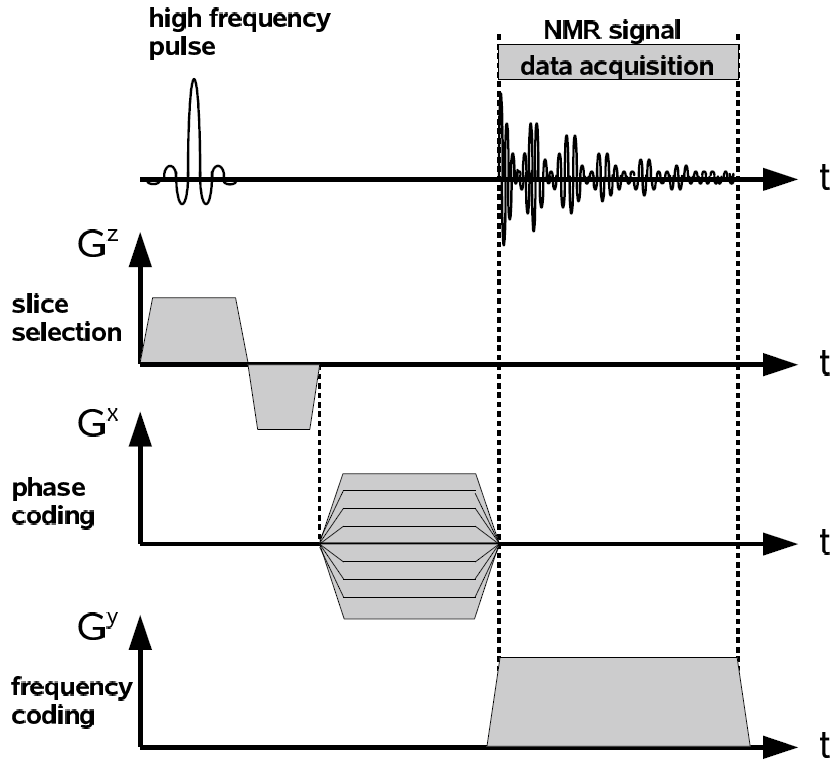
\includegraphics[width=80mm]{./Resources/2d_imaging.png}
	\caption{Pulsfolge zur Aufnahme eines zweidimensionalen Bildes. \autocite{skript}}
	\label{fig:2d_imaging}
\end{figure}

\subsubsection{Durchführung und Auswertung}

In diesem Versuchsteil verwenden wir den \textsf{Bruker$^{\textregistered}$ NMR analyzer mq7.5}, ein professioneller NMR-Analysator für ein- und zweidimensionale Messungen. Für die Analyse der aufgenommenen Bilder steht uns eine kommerzielle Software der Firma \textsf{Bruker$^{\textregistered}$} zur Verfügung.

\paragraph{Eindimensionale Bildgebung}

Wir beginnen unsere Messung mit verschiedenen Wasser- und Ölproben, die wir in vertikaler Richtung (y-Richtung) scannen.

\begin{itemize}
	\item Ein Glaszylinder wird \SI{15}{mm} hoch mit Öl gefüllt. Wie erwartet erhalten wir ein rechteckiges Signal.
	\item Ein Glaszylinder wird \SI{50}{mm} hoch mit Wasser gefüllt. Es entsteht wieder ein rechteckförmiges Signal, diesmal breiter und von höherer Intensität, da die Dichte der Wasserstoffatome größer ist als in Öl. Aufgrund der Inhomogenität des Magnetfeldes treten nichtlineare Effekte auf. Dies äußert sich in einer Krümmung des Signals in einem Bereich, der eigentlich ein konstantes Signal liefern sollte. Daher sollte die Probe dort positioniert werden, wo diese Inhomogenitäten nicht auftreten (um den Nullpunkt: $\pm$ \SI{5}{mm}).
	\item Es wird der Glaszylinder mit der scheibenförmigen Teflonstruktur eingesetzt. Da Teflon kein NMR-Signal erzeugt, sind im Signal fünf Vertiefungen zu erkennen, für jede Scheibe eine. An diesen Stellen wird das Wasser stärker verdrängt, weshalb das Signal schwächer ist.
	\item Wir untersuchen den Versickerungsprozess von Öl in Sand hinsichtlich der Frage, ob es sich um einen \emph{Diffusionsprozess} handelt. Dazu befüllen wir den Glaszylinder mit einer \SI{15}{mm} hohen Sandschicht, auf der eine \SI{4}{mm} hohe Ölschicht platziert wird. Wir messen die zeitliche Entwicklung der vertikalen Verteilung des Öls im Sand (siehe Abbildung \ref{fig:oel_diff}).

	Diffusion folgt dem zweiten Fickschen Gesetz (eindimensionaler Fall):
	\begin{equation}
		\frac{\partial c}{\partial t} = D \frac{\partial^2 c}{\partial x^2}
	\end{equation}
	Wir betrachten eine Stelle im Sand. Hier gilt stets $\tfrac{\partial c}{\partial t} > 0$ und $D > 0$, wobei $D$ der Diffusionskoeffizient ist. Daraus folgt, dass $\tfrac{\partial^2 c}{\partial x^2} > 0$, d.h. alle Konzentrationskurven im Sand sollten konvex sein.

	In unserem Fall jedoch sind alle alle Kurven in beiden Abbildungen \ref{fig:oeldiff_chinchilla} und \ref{fig:oeldiff_papa} konkav. Dementsprechend kann es sich nicht um Diffusionsprozesse handeln, sondern um normale Versickerungsprozesse.
\end{itemize}

\begin{figure}[htbp]
	{
		\centering
		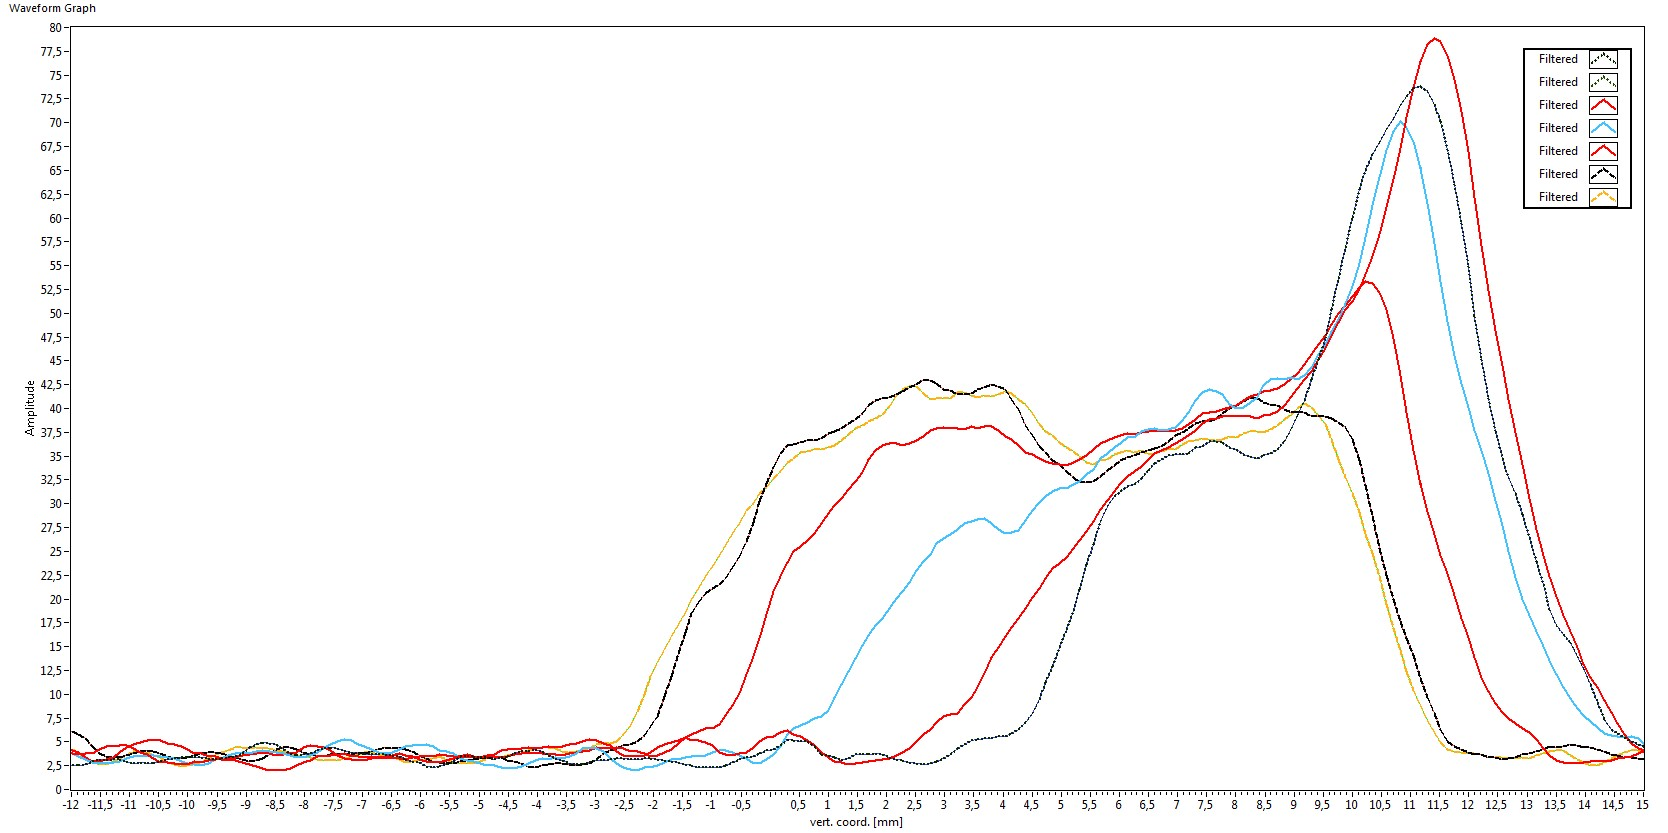
\includegraphics[width=.8 \linewidth]{./Resources/Teil_3/oeldiff_chinchilla.jpg}
		\subcaption{Chinchillasand, feinkörnig}
		\label{fig:oeldiff_chinchilla}
	\vspace{1cm}
	
		\centering
		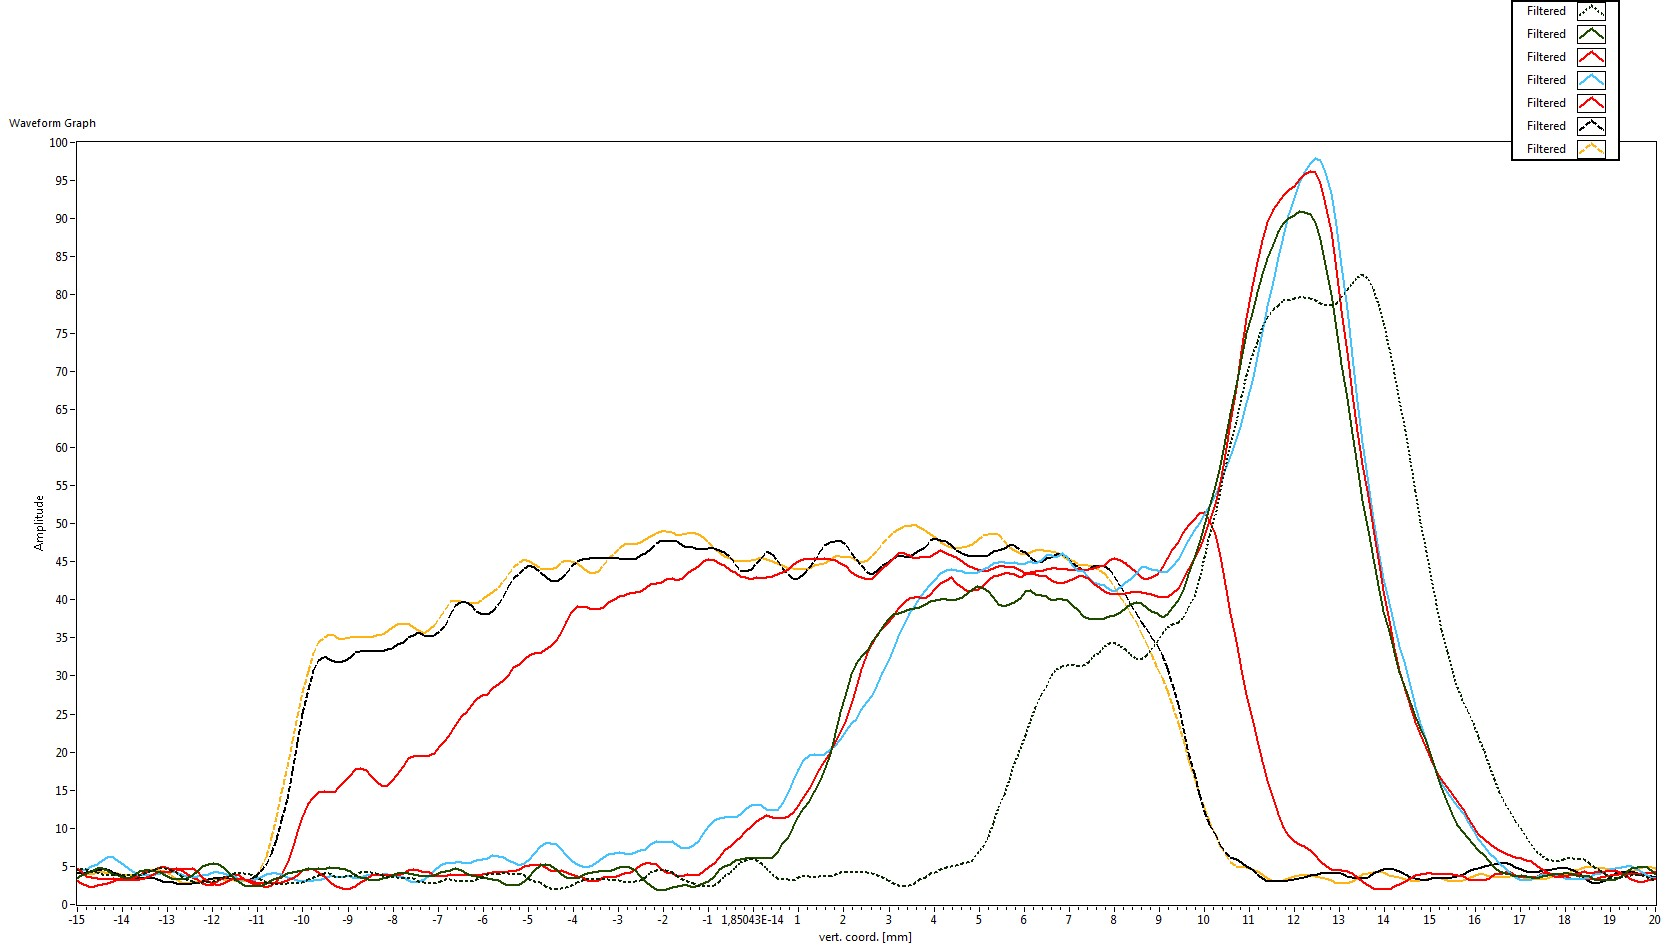
\includegraphics[width=.8 \linewidth]{./Resources/Teil_3/oeldiff_papa.jpg}
		\subcaption{Papageiensand, grobkörnig}
		\label{fig:oeldiff_papa}
	}	
		\caption{Zeitliche Aufnahmen des Versickerung von Öl im Sand. Die größere Porosität vom Papageiensand führt zu einer rascheren Versickerung (oben).}
		\label{fig:oel_diff}
	
\end{figure}

\paragraph{Zweidimensionale Bildgebung}

Folgende Messungen werden mittels 2-D-Fouriermethode durchgeführt:

\begin{itemize}
	\item Es wird ein Glaszylinder mit \SI{15}{mm} Öl befüllt und ein horizontaler Ausschnitt gewählt (Abbildung \ref{fig:2d_oel_hori}). Wie erwartet sehen wir eine mehr oder minder homogene Kreisscheibe. Ein vertikaler Ausschnitt von links nach rechts ergibt ein Rechteck, an dem unten die Wölbung des Glaszylinders und oben der Meniskus aufgrund der Oberflächenspannung sichtbar ist (Abbildung \ref{fig:2d_oel_vert}).
	\item Das Bild der PFTE-Struktur sieht auch wie erwartet aus (Abbildung \ref{fig:2d_teflon}). Da Teflon unsichtbar für unser Gerät ist, wird es schwarz dargestellt.
\end{itemize}

Bei den organischen Proben gibt die Helligkeit Aufschluss über den Wasser- bzw. Ölgehalt der Probe. Helle Stellen enthalten viel Wasser oder Öl, weshalb sie ein starkes Signal erzeugen. 

\begin{itemize}
	\item Bei der Olive (Abbildung \ref{fig:2d_olive}) ist der Stein gut zu erkennen. Er besteht aus einer trockenen Schale und enthält im Inneren den Keimling, der viel Feuchtigkeit und Öle enthält. Um den Kern ist das ölhaltige Fruchtfleisch angesiedelt. 
	\item Die Schale der Erdnuss (Abbildung \ref{fig:2d_erdnuss}) ist sehr trocken und taucht daher im NMR-Bild nicht auf. Die untere Erdnuss ist gerade so ausgerichtet, dass der Luftspalt zwischen den beiden Hälften sichtbar ist. Am unteren Ende befindet sich der Keimling, weshalb dort viel Öl vorhanden ist.
	\item In Ermangelung einer Staudensellerie mussten wir auf eine Scheibe einer Aloe vera zurückgreifen (Abbildung \ref{fig:2d_aloevera}). Man kann gut die Querschnittsform der beiden Stücke erkennen. Der Stofftransport findet in der äußeren Schicht statt, was am hellen Rand erkennbar ist.
\end{itemize}

\begin{figure}[H]
	\centering{
	\parbox{0.48\textwidth}{
		\centering
		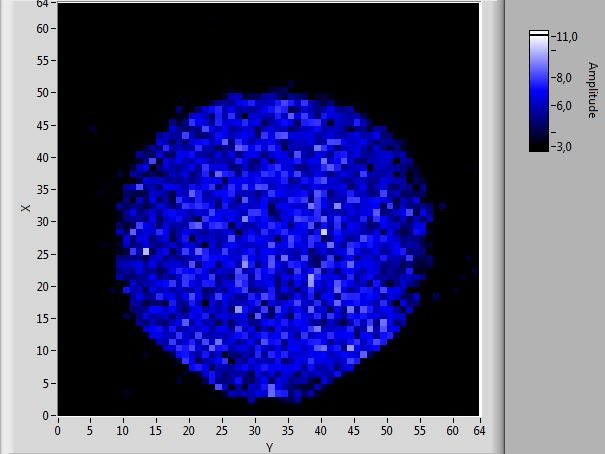
\includegraphics[width=1.0 \linewidth]{./Resources/Teil_3/oel_horizontal.JPG}
		\subcaption{Glaszylinder mit Öl, horizontaler Schnitt}
		\label{fig:2d_oel_hori}}
	\hfill  
	\parbox{0.48\textwidth}{
		\centering
		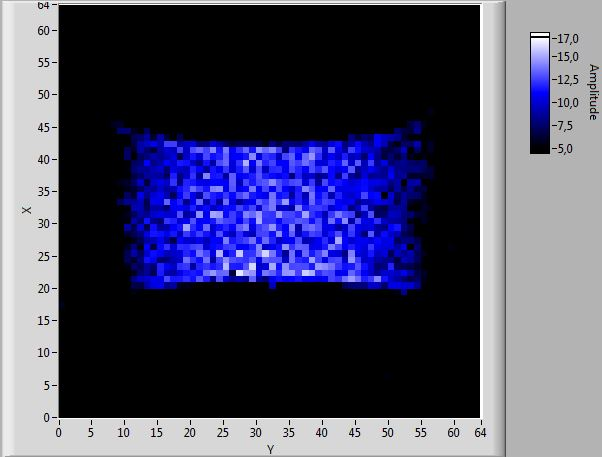
\includegraphics[width=1.0 \linewidth]{./Resources/Teil_3/oel_vert.JPG}
		\subcaption{Glaszylinder mit Öl, vertikaler Schnitt}
		\label{fig:2d_oel_vert}}
		
	\bigskip
		
	\parbox{0.48\textwidth}{
		\centering
		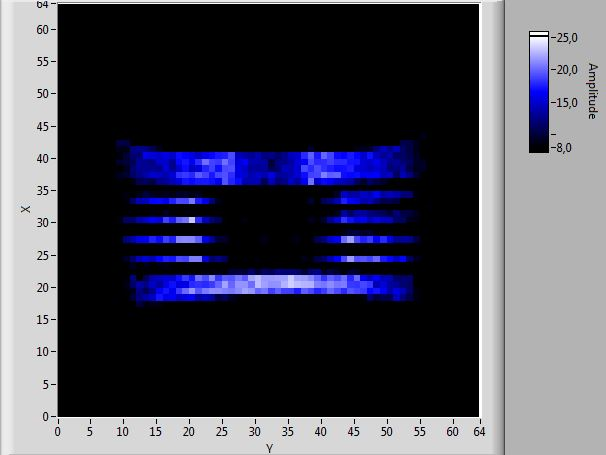
\includegraphics[width=1.0 \linewidth]{./Resources/Teil_3/ptfe_vert.JPG}
		\subcaption{Teflon-Struktur}
		\label{fig:2d_teflon}}
	\hfill  
	\parbox{0.48\textwidth}{
		\centering
		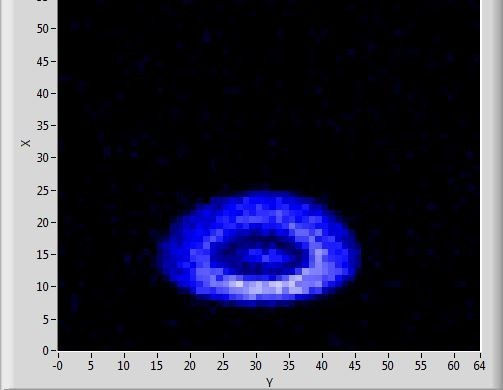
\includegraphics[width=1.0 \linewidth]{./Resources/Teil_3/olive_2d.JPG}
		\subcaption{Olive}
		\label{fig:2d_olive}}
		
	\bigskip
	
	\parbox{0.48\textwidth}{
		\centering
		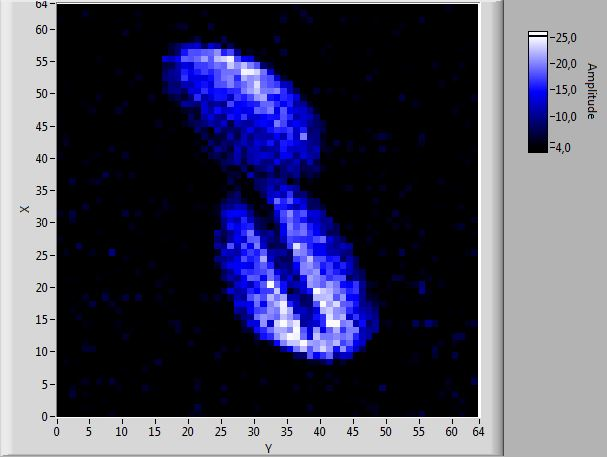
\includegraphics[width=1.0 \linewidth]{./Resources/Teil_3/peanut_shell.JPG}
		\subcaption{Zwei Erdnüsse in der Schale}
		\label{fig:2d_erdnuss}}
	\hfill  
	\parbox{0.48\textwidth}{
		\centering
		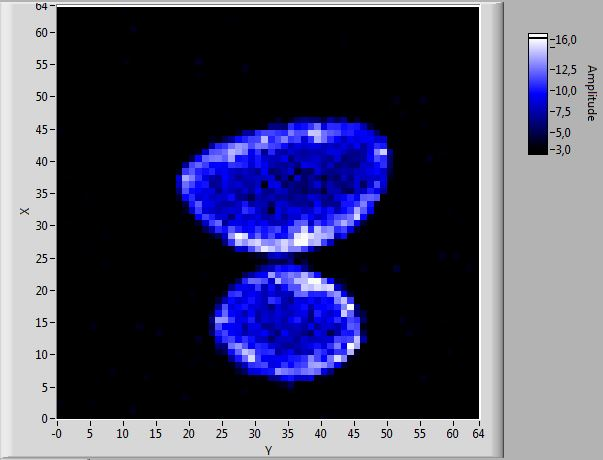
\includegraphics[width=1.0 \linewidth]{./Resources/Teil_3/aloevera_2d.JPG}
		\subcaption{Aloe vera im Querschnitt}
		\label{fig:2d_aloevera}}
		
		}	
		\caption{Zweidimensionale Aufnahmen von verschiedenen Objekten}
		\label{fig:2d_main}
	
\end{figure}


\section{Zusammenfassung und Fazit}

Im ersten Versuchsteil haben wir die Grundlagen der Kernresonanzspektroskopie anhand eines älteren, aber vielleicht gerade deswegen sehr einfach zugänglichen Spektrometers experimentell kennengelernt. Nach der Kalibration des Systems wurden an zwei unterschiedlich stark verdünnten Gd-Proben Messungen der Relaxationszeiten $T_1$ und $T_2$ durchgeführt. Durch die Unterschiede zwischen den beiden Zeiten an sich als auch zwischen den Proben konnten die theoretischen Erwartungen an die Spin-Gitter- und Spin-Spin-Wechselwirkung direkt überprüft werden. 

Im zweiten Versuchsteil wurde dann bereits eine sehr eindrückliche Anwendung des NMR-Spektrometers demonstriert. Mithilfe der chemischen Verschiebung konnten chemische Verbindungen anhand ihrer jeweiligen funktioniellen Gruppen bestimmt werden. Dabei wurde eine erstaunliche Energieauflösung von $10^{-13}~\mathrm{eV}$ erzielt!

Abschließend wurde mithilfe eines neueren Analyzers die Möglichkeit untersucht, Kernresonanzspektroskopie zur Bildgebung einzusetzen. In mehreren ein- und zweidimensionalen Messungen konnten zahlreiche organische und anorganische Objekte und deren innere Zusammensetzung betrachtet werden. Die korrekte Positionierung der Probe innerhalb der Analyseröhre war dabei kritisch, was in der Durchführung schnell zeitaufwendig wurde, da jede Messung erst automatisch kalibriert werden musste. Im Rahmen der Versuchsdauer mussten ebenso Abstriche bei der Auflösung gemacht werden, da insbesondere im zweidimensionalen Fall jede zusätzlich aufgenommene Zeile die Messzeit erheblich steigerte. Nichtsdestotrotz konnten wir auch bei den organischen Proben die inneren Strukturen ausreichend gut erkennen und so z.B. bei der Olive die Ausprägung von Kern und Fruchtfleisch vergleichen sowie bei der Aloe-Vera Pflanze die Transportkanäle erkennen.

Zusammenfassend bot dieser Versuch einen spannenden Einblick in die Technik der Kernresonanzspektroskopie, die heute in perfektionierter Form aus dem klinischen Alltag und zahlreichen anderen Bereichen nicht mehr wegzudenken ist. Bereits mit unseren einfachen Versuchsaufbauten haben wir mitunter erstaunlich genaue Messergebnisse erzielt, und durch einfache Verbesserung ließe sich die Genauigkeit sicherlich auch noch steigern.

\printbibliography

\end{document}
